\documentclass[a4paper,12pt,titlepage, twoside, openright, cleardoubleempty]{scrreprt} %page-size, letter-size, with title, is an article

\usepackage[ngerman, english]{babel} %all inserted strings will be german
\usepackage{a4wide} %for better viewing of a4 pages
\usepackage{amsmath}
\usepackage{amssymb}

\usepackage{ntheorem}

\usepackage[T1]{fontenc} %T1-encoded fonts: auch Wörter mit Umlauten trennen
\usepackage{lmodern}
\usepackage[latin1]{inputenc} %letter-style like input � or � possible

\usepackage{vmargin} %Seitenränder einstellen leichtgemacht
\usepackage{fancyhdr} %definiere einfache Headings (mindestens V 1.99c notwendig)

\usepackage{float} %to be able to insert graphics with [H] Options
\usepackage{makeidx} %so the \printindex works

\usepackage{pst-all} %pretty good drawing kit

\usepackage{listings}

\usepackage[vlined,boxed]{algorithm2e}

\usepackage[normalem]{ulem}

\usepackage{textgreek}

\lstset{basicstyle=\ttfamily,breaklines=true}

\usepackage{remreset} %folgende Zeilen benötigt, damit Fußnoten sich nicht zurücksetzen bei neuem Kapitel
\makeatletter
\@removefromreset{footnote}{chapter}
\makeatother 

\lstset{breaklines=true}
\lstset{basicstyle=\ttfamily}
\lstset{language=Java}
\lstset{tabsize=4}

\setcounter{secnumdepth}{3}% Numerierung auch für \subsubsection
\setcounter{tocdepth}{3}% nimm auch \subsubsections ins Inhaltsverz. auf

\clubpenalty = 10000
\widowpenalty = 10000
\displaywidowpenalty = 10000

\setpapersize{A4}
\setmarginsrb{3cm}{1cm}{3cm}{1cm}{6mm}{7mm}{5mm}{15mm}

%% Stil
\parindent 0cm                     % Absatzanfang wird nicht eingerückt
\parskip1.5ex plus0.5ex minus0.5ex % Abstand zwischen zwei Absätzen

\newtheorem{Def}{Definition}

\pagestyle{fancy}
\renewcommand{\chaptermark}[1]{\markboth{\thechapter.\ #1}{}}
\fancyhf{} % clear all header and footer fields
\fancyhead[LE,RO]{{\headfont\thepage}} % left/right header for even/odd pages
\fancyhead[LO]{\headfont\nouppercase{\rightmark}} % header for left side (odd)
\fancyhead[RE]{\headfont\nouppercase{\leftmark}} % right header for even pages
\renewcommand{\headrulewidth}{0.5pt} % head rule
\renewcommand{\footrulewidth}{0pt} % no rule
% plainstyle
\fancypagestyle{plain}{%
\fancyhf{} % clear all header and footer fields
\renewcommand{\headrulewidth}{0pt}
\renewcommand{\footrulewidth}{0pt}
}

\usepackage[pdftex]{graphicx}
\usepackage[pdftex,
bookmarksnumbered,
bookmarks,
bookmarksopen,
bookmarksopenlevel=1,
hypertexnames,
breaklinks,
]{hyperref}
\hypersetup{
pdftitle    = {Titel},
pdfsubject  = {...},
pdfauthor   = {},
pdfkeywords = {},
colorlinks  = {false},
linkcolor   = {blue},
citecolor   = {cyan}
}
\pdfcompresslevel=9
\pdfinfo{
/CreationDate (D:2015 11 24 00 00 00) % year(4) month(2) day(2) hour(2) minute(2) second(2)
/ModDate      (D:2015 11 24 00 00 00) % modification date
}

%%%%%%%%%%%%%%%%%%%%%%%%%%%%%%%%%%%%%%
%%%%%%%%%%%%%%%%%%%%%%%%%%%%%%%%%%%%%%
%%%%%%%%%%%%%%%%%%%%%%%%%%%%%%%%%%%%%%
%%% Hier die richtige Trennung von Wörtern festlegen, die Latex sonst 
%%% falsch trennt.
%%%%%%%%%%%%%%%%%%%%%%%%%%%%%%%%%%%%%%
%%%%%%%%%%%%%%%%%%%%%%%%%%%%%%%%%%%%%%
%%%%%%%%%%%%%%%%%%%%%%%%%%%%%%%%%%%%%%
\hyphenation{Media-annotation}


\makeindex %must be before "begin{document}
\begin{document}
\graphicspath{{pics/}}

\pagestyle{empty}

\pagenumbering{roman}

%%%%%%%%%%%%%%%%%%%%%%%%%%%%%%%%%%%%%%
%%% Titelseite
%%%%%%%%%%%%%%%%%%%%%%%%%%%%%%%%%%%%%%
\selectlanguage{ngerman}
\begin{titlepage}
\begin{singlespacing}
\begin{center}
\begin{flushleft}
	University of Passau\\
	Faculty of Computer Science and Mathematics
\end{flushleft}

\begin{center}

\vspace{1.0cm}


\includegraphics[width=7cm]{figures/uni-logo.png}

\vspace{2.5cm}


\Large{Bachelor thesis}

\vspace{1.0cm}

\begin{doublespace}
\textsf{{\Huge\textbf{\thetitle}}}
\end{doublespace}

\vspace{1.0cm}

{\bfseries \Large{\theauthor}}

\vfill
\end{center}

%%% oder:
% \date{<schreib_irgendwas_rein>}


\vspace{3.0cm}

\normalsize
\begin{flushleft}
\begin{tabular}{ll}
\multicolumn{2}{l}{Bachelor thesis}\\
\multicolumn{2}{l}{Chair of Distributed Information Systems}\\
\multicolumn{2}{l}{Faculty of Computer Science and Mathematics}\\
\multicolumn{2}{l}{University of Passau}\\
\\
%%%%%%%%%%%%%%%%%%%%%%%%%%%%%%%%
%%% Falls Diplomarbeit - bei BA nur ein Gutachter im Moment
%%%%%%%%%%%%%%%%%%%%%%%%%%%%%%%%
Examiner: & Prof. Dr. Harald Kosch \\
Supervisor: & Armelle N. Ndjafa
\end{tabular}
\end{flushleft}

\parbox{\linewidth}{\hrule\strut}

\thedate

%\dedication{Widmung}
\end{center}
\end{singlespacing}
\end{titlepage}

\pagestyle{fancy}
\selectlanguage{english}

%%%%%%%%%%%%%%%%%%%%%%%%%%%%%%%%%%%%%%
%%% Kurzfassung (wenn möglich auf Englisch, ansonsten Deutsch)
%%%%%%%%%%%%%%%%%%%%%%%%%%%%%%%%%%%%%%
\chapter*{Abstract}

Health care faces the problem of dealing with a vast amount of heterogenous data, that isn't easily accessible. Classical data integration approaches need a global schema before queries on the integrated data can be stated. Dataspace is a new abstraction of data management, that doesn't enforce any schema, allows data-coexistence, and needs only low upfront work for datasources thus being suitable for highly heterogeneous environments. In this thesis we present MeDSpace, a distributed system that allows to state keyword search queries over heterogeneous datasources. The presented system is a test environment for medical datasources and can be used as a starting point for creating a dataspace over multimedia datasources. The system uses medical data, but could be used for any kind of multimedia data that should be searchable by keywords.

%%%%%%%%%%%%%%%%%%%%%%%%%%%%%%%%%%%%%%
%%% Inhaltsverzeichnis
%%%%%%%%%%%%%%%%%%%%%%%%%%%%%%%%%%%%%%
\tableofcontents

\cleardoublepage %beginne neue Seitenzählung auf einer rechten Seite (ungerade Seitenzahl)

%%%%%%%%%%%%%%%%%%%%%%%%%%%%%%%%%%%%%%
%%% Tabellenverzeichnis
%%%%%%%%%%%%%%%%%%%%%%%%%%%%%%%%%%%%%%
\listoftables
\addcontentsline{toc}{chapter}{List of Tables}

%%%%%%%%%%%%%%%%%%%%%%%%%%%%%%%%%%%%%%
%%% Abbildungsverzeichnis
%%%%%%%%%%%%%%%%%%%%%%%%%%%%%%%%%%%%%%
\listoffigures
\addcontentsline{toc}{chapter}{\listfigurename}

%%%%%%%%%%%%%%%%%%%%%%%%%%%%%%%%%%%%%%
%%% Diese beiden Zeilen werden für Doppelseitigen Ausdruck benötigt und
%%% damit erst nach dem Inhaltsverzeichnis die Seiten gezählt werden.
%%%%%%%%%%%%%%%%%%%%%%%%%%%%%%%%%%%%%%
\cleardoublepage
\pagenumbering{arabic}

%%%%%%%%%%%%%%%%%%%%%%%%%%%%%%%%%%%%%%
%%% Ab hier beginnt die eigentliche Arbeit.
%%%
%%% 2 Varianten:
%%%     - entweder einzelne Kapitel mit include einbinden (bessere Übersicht)
%%%     - oder den ganzen Text einfach reinschreiben (unübersichtlich)
%%% Wie es gemacht wird spielt fürr den eigentlichen Output keine Rolle.
%%%%%%%%%%%%%%%%%%%%%%%%%%%%%%%%%%%%%%
%%%% Part dient dazu, zb. die Arbeit nochmal zu Gliedern (Einleitung, Theorieteil, ...)
\part{Part}

% neues Kapitel
\chapter{Chapter}

Always make a short intro to chapters or sections.

%neue Section
\section{Section}
\label{erstesLabel}

some intro words \dots

% NICHT TIEFER ALS SUBSECTION!!!
\subsection{SubSection}
\label{zweitesLabel}

First label was set in section \ref{erstesLabel} - the second in section \ref{zweitesLabel}.

Remember: Always reference any figures or tables within the prose text!

A reference will be done like this: \cite{keyToBibEntry}

Do not cite things like Wikipedia, Slides, etc (only Books and scientific papers allowed - or W3C Recommendations \cite{w3c_example} and articles on trusted sites marked with a date and an corresponding author)

Please code URLs like this: \url{http://www.google.de}

If you name projects like A.I.R\footnote{\url{https://www.dimis.fim.uni-passau.de/iris/index.php?view=air} -- last checked: \today} or Eclipse\footnote{\url{http://www.eclipse.org/} -- last checked: \today} or whatever, use footnotes to cite the URL.

%Example Figure
\begin{figure}[H]
	\begin{center}
		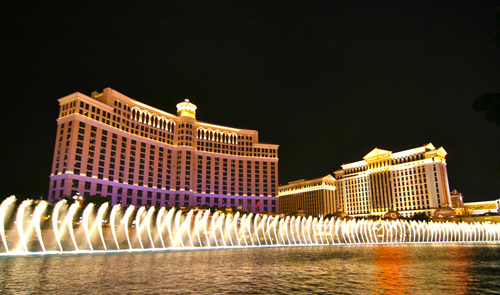
\includegraphics[width=0.75\textwidth]{holiday.png}
	\end{center}
	\caption{After the thesis it's time for holiday}
	\label{labelToRef}
\end{figure}

%Example Itemize
\begin{itemize}
	\item item 1
	\item item 2
	\item lala
\end{itemize}

%Example Description
\begin{description}
	\item[item 1] is needed in order to blabla
	\item[item 2] defines blabla
	\item[lala] lala
\end{description}

% Example Definition
\begin{Def}[Title]
\label{key}
Description \dots
\end{Def}

% Example Table
\begin{table}[H]
\begin{center}
\caption{Caption of the table}
\label{lalala}
\begin{tabular}{| l | l |}
\hline
first column & second column \\
\hline
\hline
\dots & \dots \\
\hline
\dots & \dots \\
\hline
\end{tabular}
\end{center}
\end{table}

\begin{procedure}[ht]        
\caption{Greedy Heuristic()} 
\label{greedy}        
\KwData{request profile $Q$, backends $B$} 
\KwResult{allocation schema}

sort(request profile $Q$) according cost function $c_S$ descending \; 

\ForEach{$C \in Q$}{

   \ForEach{$b \in B$}{
      \eIf{$b.free\_capacity > 0$} {
      $UNION \leftarrow b.relations \cup C.relations$\;
      $INTERSECT \leftarrow b.relations \cap C.relations$\;
      ${diff}[C,b] \leftarrow c_S(INTERSECT) - c_S(UNION)$\;
      }
      {$diff[C,b] \leftarrow -\infty$;}
   }
   
   \While{$C.rest\_workload > 0$}{
      
      $b \leftarrow b \in B \mbox{ where } diff[C,b]  \mbox{ maximal}$\;
      
      $workload\_for\_b \leftarrow \min({b.free\_capacity, C.rest\_workload})$\;
      
      $b.add(C , workload\_for\_b)$\;
      
      $C.rest\_workload \leftarrow C.rest\_workload - workload\_for\_b$\;
      
      
      ${diff}[C,b] \leftarrow -\infty$;
      
   }
}
\end{procedure}


\chapter{Introduction}

In the fields of medicine every year a vast amount of (digital) data is produced, that usually is very complex \cite[p. 1]{ASurveyOnDataMiningApproachesForHealthcare}. 
The data in the healthcare sector are combinations of classical text files, images, audio, and videos that is used in combination. Thus the data meets the definition of multimedia data, which is exactly a conjunction of multiple kinds of data that is used to present modal information \cite[p. 2]{DBLP:journals/corr/abs-1102-5769}.

Health data is also highly heterogeneous (e.g. different file formats) and and often requires lots of tools to work with.\cite[p. 1]{Raghupathi2014}. In summary, searching data and working with it isn't a straightforward process, and indeed causes many costs.

As a result, the ability to easily access the data would be beneficial for both, research and healthcare institutions \cite[p. 2]{Raghupathi2014}:
\begin{itemize}
	\item Lower Costs
	\item Detecting diseases at early stages
	\item Simplified collaboration
	\item Healthcare fraud detection
\end{itemize}


The above mentioned benefits were originally stated for Big Data Analysis and Data Mining. 
Both research fields require as a first step to integrate the data of different datasources into one data integration system. Creating a data integration system for the healthcare sector would not only be reasonable, but offers lots of necessary benefits to the whole healthcare system.

But there is another option, the so-called dataspace concept, that doesn't semantically integrate data before it is able to provide its services, and follows a data co-existence approach. Data co-existence means that data from a query result isn't fully integrated. So it is allowed e.g. that semantical equal data is presented differently. Duplicates  in a query result are thus acceptable.
Data co-existence facilitates work with heterogeneous data and many schemas. As heterogeneity is a first-class citizen in a dataspace, it is also useful for integrating multimedia data. 
These are attractive properties and reason in this work for to follow the dataspace concept . The dataspace concept was introduced in 2005 as a vision \cite{Franklin:2005:DDN:1107499.1107502}. Yet, until today no fully fledged dataspace implementation was presented.

%But to the time of this writing, no fully fledged dataspace implementation was presented. 

In this thesis we present a distributed environment to state keyword search queries on multiple heterogeneous multimedia medical datasources. We called this system MeDSpace which is an abbreviation for \emph{Medical Dataspace}. The system could be used as a base for implementing a fully fledged dataspace or for any system, that needs keyword search functionality on multiple heterogeneous (distributed) datasources. Despite the research of dataspaces is very active, they often cover only text data ignoring the properties of multimedia data \cite{6167826}. This is another reason, why we explicitly chose multimedia data.

There should be noted, that although we use medical data for test data of the system to be presented, the system itself isn't restricted to any kind of particular data.

The content of the thesis is structured as follows: In the first chapters we will present foundation knowledge of data integration and dataspaces. Then we will cover related work and reference projects. In chapter 5 the structure and the provided services of MeDSpace is presented and in chapter 6 the implementation of our system is described in detail. At the end, in chapter 6 we will give some outlook, suggestions, and possible improvements to the system. 

\chapter{Foundation in Data integration}
\chapter{Motivation}
\section{Information Integration}

Information integration addresses to integrate existing databases. Synonyms for information integration are information fusion, data consolidation, data cleansing or data warehousing. The goal of information integration is almost always to simplify the access to a range of existing information systems through a central, integrated component with a unified interface for users and applications. Therefore, integrated information systems provide a unified view on the data sources. Existing information systems can be diverse: Classical relational database systems, files, data accessed by web services or HTML formulas, data generating applications or even other integrated information systems. (from \cite[p. 3-4]{DBLP:books/dp/LeserN2006}, own translation).\\
Today, data is classified into three diverse categories. Structured data like it is stored in relational databases, have a predefined structure through a schema.
Semi-structured data also have a schema, but they can deviate from the schema. An example of semi-structured data is a XML file without an accompanying XML schema. The third class is unstructured data and contains, as the name implies, no given structure. Typical unstructured data is natural language text.
(from \cite[p. 17]{DBLP:books/dp/LeserN2006}, own translation).\\
If we speak of diverse information systems we usually mean heterogeneous systems. Heterogeneity exists among data sources as well as between data sources and the integrated system. In most of all integrated information systems only the latter heterogeneity matters, as data sources often do not communicate among themselves. 
To bridge heterogeneity, it is obviously necessary to translate queries and to implement missing functionality in the integrated system. Table \ref{kinds-of-heterogeneity} shows an overview of existing kinds of heterogeneity (from \cite[p. 60/61]{DBLP:books/dp/LeserN2006}, own translation).

\begin{table}[]
\centering
\caption{Kinds of heterogeneity}
\label{kinds-of-heterogeneity}
\begin{tabular}{|l|p{0.7\textwidth}|}
\hline
 \textbf{Technical  heterogeneity}  &  includes all problems to realize the access of the data of the data sources technically. This heterogeneity is overcome if the integrated system is able to send a query to a data source and that data source principally understands the query and produces a set of data as result.\\ \hline
 \textbf{Syntactic  heterogeneity}    &  includes problems in the illustration of information. This heterogeneity is overcome if all information meaning the same are illustrated equally.\\ \hline
 \textbf{Data model  heterogeneity} &  means problems in the presentation of data of the used data models. This heterogeneity is solved if the data sources and the integrated system use the same data model.\\ \hline
 \textbf{Structural  heterogeneity}    &  includes differences in the structural representation of information. This heterogeneity is solved if semantic identical concepts are also structural equally modeled. \\ \hline
 \textbf{Schematically  heterogeneity} &  Important special case of the structural heterogeneity, whereby there are differences in the used data model.\\ \hline
 \textbf{Semantic  heterogeneity}    &  Includes problems regarding the meaning of used terms and concepts. This heterogeneity is solved if the integrated system and the data source understand by the used names for schema elements really mean the same. Equal names means consequently equal meaning.\\ \hline
\end{tabular}
\end{table}

In general, there are two different types of information integration: The materialized integration and the virtual integration. The difference between these two approaches is as follows: At materialized integration the data to be integrated is stored  into the integrated system itself, so on a central point. The data in the data sources remains but for querying the materialized view is used. At virtual integration, the data is only transported from the data source to the integrated system while the query processing. This temporary data is then again discarded. So integration isn't done once but on each query. Of course, an integrated information system can use both principles. Such a system is called hybrid. Both types have in common that a query is processed on a global schema. For the virtual integrated system, the data only exists virtual, thus relations between data sources and the global schema have to be specified and on query time the query has to be split into into query schedules. The schedules are responsible to extract the needed information from the different data sources and subsequently merge and transform the data (from \cite[p. 86-88]{DBLP:books/dp/LeserN2006}, own translation).


\begin{table}[]
\centering
\caption{Different architectures of integrated information systems}
\label{architectures-of-integrated-information-systems}
\begin{tabular}{|l|p{0.7\textwidth}|}
\hline
 \textbf{}  &  includes all problems to realize the access of the data of the data sources technically. This heterogeneity is overcome if the integrated system is able to send a query to a data source and that data source principally understands the query and produces a set of data as result.\\ \hline
 \textbf{Syntactic  heterogeneity}    &  includes problems in the illustration of information. This heterogeneity is overcome if all information meaning the same are illustrated equally.\\ \hline
 \textbf{Data model  heterogeneity} &  means problems in the presentation of data of the used data models. This heterogeneity is solved if the data sources and the integrated system use the same data model.\\ \hline
 \textbf{Structural  heterogeneity}    &  includes differences in the structural representation of information. This heterogeneity is solved if semantic identical concepts are also structural equally modeled. \\ \hline
 \textbf{Schematically  heterogeneity} &  Important special case of the structural heterogeneity, whereby there are differences in the used data model.\\ \hline
 \textbf{Semantic  heterogeneity}    &  Includes problems regarding the meaning of used terms and concepts. This heterogeneity is solved if the integrated system and the data source understand by the used names for schema elements really mean the same. Equal names means consequently equal meaning.\\ \hline
\end{tabular}
\end{table}



\textcolor{red}{//comment!//}
\chapter{Dataspaces}
The concept of dataspaces was the first time presented in 2005 and describes a new abstraction of data management \cite[p. 27]{Franklin:2005:DDN:1107499.1107502}. 
The motivation for a new type of data management arises from the issue that rarely the data to be managed is solely stored in a convenient relational database, nor is stored in a single data model.
For a long time relational databases were the dominating choice for storing data, but this is changing, as the coming popularity of NoSQL databases indicates \cite{SQL_NOSQL_DATABASES}. Also for multimedia content, relational databases aren't always an ideal choice since they were conceptualized for structured data, whereas multimedia data can contain all types of data. Also distribution is a problem, that is difficult to handle with relational databases, since they were also designed for monolithic use-cases.
We can record that applications have to handle more and more different types of data sources and thus have to handle heterogeneous and distributed data, too.

That issue is ubiquitous and arises in enterprises, government agencies and even on everybody's PC desktop. As example par excellence serves the healthcare sector dealing with highly heterogeneous and complex data, and struggling with a continuously growing amount of data.

%As a result, developers face the challenge to deal with heterogeneous data on a low level base. Challenges are to provide search and query capabilities, enforcing rules, integrity constraints, naming conventions etc.; tracking lineage; providing availability, recovery and access control; and managing evolution of data and meta-data. That issues are ubiquitous and arise in enterprises, government agencies and even on one's PC desktop. 
As a response to this problem, the authors of \cite{Franklin:2005:DDN:1107499.1107502} postulate the concept of dataspaces and corresponding to this the  development of DataSpace Support Platforms (DSSPs). Shortly said, the latter provides an environment of cooperating Services and guaranties that enables software developers to concentrate on their specific application problem rather than taking care of returning issues in consistency and efficiency of huge, linked but heterogeneous data sets. The remarkable properties of a dataspace system are defined as follows \cite[p. 28]{Franklin:2005:DDN:1107499.1107502}:

\begin{itemize}
\item A DSSP must deal with data and applications in a variety of file formats that are accessible through many systems with different interfaces. A DSSP has to support all kinds of data in the dataspace and isn't allowed to omit any ( e.g. as DBMSs do).

\item An integrated possibility for searching, querying, updating and administration is provided by the DSSP, but the data often is also accessible and modifiable through native interfaces. Therefore DSSPs haven't full control over their data.

\item The DSSP can offer several query services, but isn't forced to return the most accurate result. Indeed,  the answers can be approximated resp. \emph{best-effort}. If some data sources e.g. are unavailable for some reason, the dataspace might use the current available data sources and creates the best possible result.

\item Whenever it is required, the DSSP has to provide tools to do tighter data integration.
\end{itemize}

Current data integration systems are essentially a natural extension of traditional databases, where queries are specified in a structured form and data is modeled in one of the traditional data models like relational or XML. The System for data integration also has exact information about how the data in the sources map to the schema used for integration. So, for data integration there is a need for large upfront effort in creating the mediated schema and the schema mappings.

Many of the services a dataspace provide, data integration and exchange systems provide, too. The main difference between these systems is that data integration systems need a semantic integration process before they can provide any services on the data. Additionally, data integration systems always have a global schema. But a dataspace is not a kind of a classic data integration approach. Initially, a dataspace doesn't semantically integrate the data. It allows data to \emph{coexist}.  The idea is to provide base functionality over all data sources, regardless of their specific integration constraints. E.g. a DSSP is able to provide a keyword search similar to a desktop file search. If more sophisticated operations are required, such as relational queries, data mining or monitoring of specific data sources, additional effort can be done to integrate the sources tighter. This incremental process is also called as \emph{pay-as-you-go} data integration.

%Dataspace Support Platforms (DSSP) shall considerable reduce this upfront effort. The system should be able to bootstrap itself and provide useful services with no human intervention. When the data management needs become clearer (through user feedback or as sources are added), the system evolves in a pay-as-you-go fashion.

%\textcolor{red}{\textbf{Stuff that has to be reorganized:}}\\
%\textcolor{red}{Following paragraph have to be moved to more suitable place!}\\
%The document ``Principles of Dataspace System'' of Alon Haley, Michael Franklin and David Meier\cite{Halevy:2006:PDS:1142351.1142352} is based on their previous work ``From Databases to Dataspaces - A New Abstraction for Information Management''\cite{Franklin:2005:DDN:1107499.1107502} where the concept of dataspaces was firstly presented, and poses specific technical challenges realizing Dataspace Support Platforms (DSSPs) relating to query answering, introspection and the benefits of human attention for improving semantic relationships within a dataspace.  
%In the following are stated the results of the above mentioned challenges:


%In the paper ``Towards Realization of Dataspaces'', written by Ibrahim Elsayed and Peter Brezany\cite{1698348}, the architecture and functionality of a Dataspace Management System(DMS) is presented. Additionally it is discussed, how grid technology of future implementations is able to support such an architecture. A DMS is a set of software programs, which controls the organization, storage and retrieval of data in a Dataspace. It also handles the security and integrity of a Dataspace.
%In the following, the architecture and the functionality requirements of a DMS will be described.   

A Dataspace should contain all information being relevant for a specific organization/task, regardless of their file format or storage location, and it should model a collection of relationships between the data sources. Therefore the dataspace is defined as a set of participants and relationships \cite[p. 29]{Franklin:2005:DDN:1107499.1107502}. 
Participants of a dataspace are individual data sources. 
Some participants support expressive query languages for querying, while others only provide limited access interfaces. 
Participants can reach from structured, semi-structured right up to unstructured data sources. Some sources provide traditional updates, some are only be appendable, while others are immutable. Further, dataspaces can be nested within each other, which means that a dataspace should be able to be a part of another dataspace.  Thus, a dataspace has to provide methods and rules for accessing its sub dataspaces.

Not every participant will provide all necessary interfaces for being able to support all DSSP features \cite[p. 29]{Franklin:2005:DDN:1107499.1107502}. 
Hence, it is necessary that data sources can be extended on various ways. E.g. a source don't store its own meta-data, so there has to be an external meta-data repository for it. 

A DSSP should also support updating data \cite[p. 29]{Franklin:2005:DDN:1107499.1107502}. Of course, the mutability of the relevant data sources determines the effects of updates.  
Other key services would be monitoring, event detection and the support for complex workflows (e.g. is desired that a calculation is done if new data arrives and that the result will be distributed over a set of data sources) \cite[p. 29]{Franklin:2005:DDN:1107499.1107502}. On a similar way a DSSP should support various forms of data mining and analysis. 
The user should be able to discover relevant datasources and to look for their completeness, correctness and recency \cite[p. 29]{Franklin:2005:DDN:1107499.1107502}. A DSSP indeed should recognise when data of the domain is incomplete. 

\section{Components and Services}

In this section we will look at the components forming a fully-fledged dataspace and the services providing these components. Figure \ref{TowardsRealizationOfDataspacesEnvironment} shows the components as they were defined in \cite{1698348}:


\begin{figure}[H]
	\begin{center}
		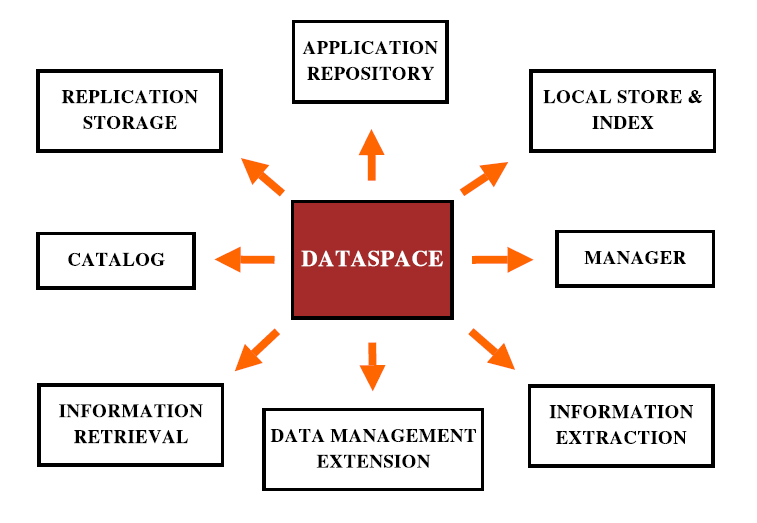
\includegraphics[width=0.75\textwidth]{figures/TowardsRealizationOfDataspaces1.png}
	\end{center}
	\caption{Environment of  a Dataspace \cite[p. 2]{1698348}}
	\label{TowardsRealizationOfDataspacesEnvironment}
\end{figure}

\uline{\textbf{Catalog:}} 
The most basic service a dataspace should provide is the cataloging of data elements of all participants. A catalog is an inventory of data resources containing all important information about every element (source, name, storage location inside the source, size, creation date, owner, etc.) of the dataspace. 
It is important that the catalog includes the schema of the source, statistics, rates of change, accuracy, completeness query answering capabilities, ownership, and access and privacy policies for each participant. 
Relationships may be stored as query transformations, dependency graphs, or even textual descriptions.The catalog is the infrastructure for the most other dataspace services. Search and query are two main services a DSSP must provide. A user should be able to state a search query and iteratively precise it, when appropriate, to a database-style query. For the dataspace approach it is a key tenet that search should be applicable to all of the contents, regardless of their formats.
The search should include both, data and meta-data. Then, it can support basic browsing over the participant's inventories. The catalog may reference a meta-data repository to separate the basic and more detailed descriptions.
It isn't a very scalable interface, but it can be used to response to questions about the presence or absence of a data element, or determine which participants have documents of a specific type. 
On top of the catalog the DSSP should have a model-management environment allowing the creation of new relationships and manipulation of existing ones.

\uline{\textbf{Information Retrieval:}} The Information Retrieval component (in \cite{Halevy:2006:PDS:1142351.1142352} stated as 'Search and Query') can be split up into queries and searches, two different methods of information retrieval, and represent together one of the main services a DSSP should support. 
Generally, queries and searches should be supported by all participants of the Dataspace, regardless of their used data model. 
It shouldn't make any difference for a user to operate on a sole database or on a Dataspace. 
A good known and simple search operation is keyword searching. 
The support of spanning such a search method over all participants is a challenging research topic: The development of methods for keyword searching on relational and XML databases was done by the data-engineering community \cite{994693, Guo:2003:XRK:872757.872762, Hristidis:2002:DKS:1287369.1287427}. 
For to support a global query functionality allowing to formulate uniform queries on all Dataspace participants, intelligent methods for interpreting and translating of queries in several languages are required. Methods for query translation were investigated by a large body of research communities \cite{Carey00xperanto:publishing, 1319983}.
In the following are listed the main requirements having to be supported by this component:

\begin{description}
\item [Query everything:]  any data item should be queryable  by the user regardless of the file format or data model. 
Keyword queries initially should be supported. 
When more information about a participant is collected, it should be possible to gradually support more sophisticated queries. 
The transition between keyword query, browsing and structured querying should be gracefully. 
Also, when answers are given to keyword (or structured) queries, the user should be able to refine the query through additional query interfaces. 

\item [Structured queries:] queries similar to database ones should be supported on common interfaces (i.e. mediated schemas) that provide access to multiple sources, or can be posed on a specific data source (using its own schema). The intention is, that answers will be obtained also from other sources (as in peer-data management systems). Queries can be posed in a variety of languages (and underlying data models), and should be translated into other data models and schemas as best as possible with the use of exact and approximate semantic mappings.

\item [Meta-data queries:] it is of essential importance that the system supports a huge variety of meta-data queries. These include (a) source inclusion of an answer or how it was derived or computed, (b) time steps provision of the data items that are included in the computation of an answer, (c) specification of whether other data items may depend on on a particular data item and the ability to support hypothetical queries. A hypothetical question would be 'What would change if I removed data item X?' (d) Querying the sources and degree of uncertainty about the answers.
Queries locating data, where the answers are data sources rather than specific data items, should be supported, too. 

\item [Monitoring:] all stated Search and Query services should also be supported in an incremental form which is also applicable in real-time to streaming or modified data sources. It can be done either as a stateless process, in which data items are considered individually, or as a statefull process. In the latter multiple data items are considered.   
\end{description}

\uline{\textbf{Local Store and Index:}} This component is responsible for caching search and query results, so that certain queries can be answered without the need of accessing the actual data sources. Furthermore it supports the creation of queryable associations between the participants. The component should try to achieve the following goals:
\begin{itemize}
\item to create efficiently queryable associations between data items in different participants. Important is here, that the index should identify information across participants when certain tokens appear in multiple ones (in a sense, a generalization of a join index)

\item to improve accesses to data items with limited access patterns. Here, the index has to be robust in the face of multiple references to real-world objects, e.g. different ways to refer to a company or person.

\item to answer certain queries without accessing actual data sources. Thus, the query load is reduced on participants which cannot allow ad-hoc external queries. 
  
\item to support high availability and recovery   
\end{itemize}

The index has to be highly adaptive to heterogeneous environments. It should take as input any token appearing in the dataspace and return the location at which the token appears and the roles at each occurrence. Occurrences could be a string in a text file, element in file path, a value in a database, element in a schema, or tag in a XML file. 

\uline{\textbf{Discovery Component:}} This component (not listed in Figure \ref{TowardsRealizationOfDataspacesEnvironment}) locates participants in a dataspace, creates relationships between them, and helps administrators to refine and tighten these relationships. For each participant the component should perform an initial classification according to the participant's type and content. The system should provide an environment for semi-automatically creating relationships between existing participants and refining and maintaining existing ones. This involves both, finding which pairs of participants are likely to be related, and then proposing relationships which a human can verify and refine. The discovery component should also monitor the content in order to propose additional relationships in the dataspace over time.  

\uline{\textbf{Data Management Extensions:}} This component (in \cite{Halevy:2006:PDS:1142351.1142352} stated as \textit{Source Extension Component}) provides possibilities to improve low-level working Dataspace components. All these base components have only limited data management capabilities. It is a task of a DSSP to provide additional functionality such as backup, recovery and replication. Some participants may not provide significant data management functions. For example, a participant might be no more than departmental document repository, perhaps with no services than weekly backups. A DSSP should support to enrich such a participant with additional capabilities, such as a schema, a catalog, keyword search and update monitoring. It may be necessary to provide these extensions locally, as there might exist applications or workflows that assume the current formats or directory structures.	
This component also supports ``value-added'' - information held by the DSSP, but not present in the initial participants. Such information can include ``lexical crosswalks'' between vocabularies, translation tables for coded values, classifications and ratings of documents, and annotations or linked attached data set or document contents. Such information must be able to span participants in order to link related data items.\\

\uline{\textbf{Information Extraction:}} The world-wide web has become a large data container by now. For allowing to postprocess data obtained from the web, techniques for web information extraction, extracting relevant information from semi-structured web pages should be supported. For further processing extracted content has to be converted to structured data, and saved locally. Non structured web documents have first to be classified using text mining techniques, which organize the parsed documents into groups with the help of ontologies \cite{conf/wise/HeQZW04}. Based on these ontologies a keyword search is able to find individual documents. Structured documents allow easier access and integration due to the rich semantically information included in the data representation.\\

\uline{\textbf{Manager:}} In order to realize the above mentioned functionality, a central component managing the system and interacting with the user is needed. Alongside user authentication, right assignments and other services, this manager component is responsible for communicating with all participants. Thus, this component serves as an interface between the users and the participants of the Dataspace.\\

\uline{\textbf{Replication Storage:}} Allows to copy participant data in order to increase its access time. This results in high availability, and high recovery is supported.\\

\uline{\textbf{Application Repository:}} With this component the user is able to share data analysis tools, domain specific models, evaluations, etc., which can be applied to the (available) data of the Dataspace.\\


\section{Query answering}

In a dataspace, queries might be posed in a wide range of different languages \cite[p. 3]{Halevy:2006:PDS:1142351.1142352}. But most of the activities will properly begin with a keyword search, but it might also be common to see queries as a result of a form (which results to queries with several selectable predicates). More complex queries arise when a user interacts deeper with a certain data source. If it isn't explicitly stated, it is usual, that a user is likely to believe that a query considers all relevant data in a dataspace, regardless of the used data model or schema. Even if a query is posed to a data source, it is implicitly expected that the system considers the data of other sources, as well. If additional answers are desired, one has to do transformations on the schema and the data model.

\textbf{Challenges of answer querying}

Answers corresponded to queries of a dataspace are different from traditional queries in several ways. In the following we list challenges a dataspace has to deal with \cite[p. 3-4]{Halevy:2006:PDS:1142351.1142352}:

\begin{itemize}
\item \textbf{Ranking}: Queries are typically sorted by their relevance, similar to a web search engine. Ranking is necessary not only for keyword search, but also for structured queries, when transitions to other data sources should be approximated.  

\item \textbf{Heterogenity}: Answers will come from many sources and will differ in their used data model and schema. The Ranking has to manage heterogeneity, too.

\item \textbf{Sources as answers}: In addition to base elements (e.g. documents or tuples), a DSSP should be able to provide sources, as well. This means that it returns links to locations where additional answers can be found.

\item \textbf{Iterative queries}: Normally, the interaction with a dataspace can't be reduced to the process of posing  a sole query and getting an answer to it. Instead, a user is involved in an information finding task that requires a sequence of queries, each being a refinement or modification on the previous ones.

\item \textbf{Reflection}: It is expected, that a DSSP reflects on the completeness of its coverage and the accuracy of its answers. 
\end{itemize}


\section{Uncertainty in Dataspaces}
 
In the paper ``Data Modeling in Dataspace Support Systems'' \cite{DBLP:conf/birthday/SarmaDH09}, the authors face the issue of uncertainty in dataspaces. In their view, a dataspace needs to model uncertainty in its core. In their work, they described the concepts of probabilistic mediated schemas and probabilistic mappings as enabling concepts for DSSPs. With this foundation, it is possible to completely bootstrap a pay-as-you-go integration system. 
In order to develop DSSPs, it is impossible to rely on the same data modeling paradigms data integration systems use. One cannot assume, that the mediated schema is given in advance and that the schema mappings between the sources and the mediated schema will be accurate. Therefore the authors argue that uncertainty has to be considered in the mediated schema and in the schema mappings.

Now, we discuss the different kinds of uncertainty, that can arise in a datasapce \cite[p. 123]{DBLP:conf/birthday/SarmaDH09}:

\begin{itemize}
\item \textbf{Uncertain mediated schema}: The set of schema terms in which queries are posed is called the mediated schema. Not necessarily they cover all the attributes in any source, it cover rather the aspects of the domain that the developer of the application wishes to expose to the user. For several reasons uncertainty happens in the mediated schema. First, if the mediated schema is derived from the data sources during bootstrapping, there will be some uncertainty about the results. When domains are broad, there will be also some uncertainty about how to model them, because in general, there will be overlappings in different topics. 

\item \textbf{Uncertain schema mapping}: Schema mapping defines the semantic relationships between the terms in the sources and the terms used in the mediated schema. Although, schema mappings can be inaccurate. In a dataspace, many of the initial schema mappings are properly automatically derived, and therefore they may inaccurate. In general, it is impossible to create and maintain precise mappings between data sources. 

\item \textbf{Uncertain data}: Some of the data may be obtained by automatism as data sources may not always be structured well. Additionally, unreliable or inconsistent data may be contained in systems with many sources.

\item \textbf{Uncertain queries}: Properly, much of the early interaction with a dataspace will be done through keyword queries as the users aren't aware of a (non-existent) schema. The queries have to be translated into some structured form so they can be reformulated with respect to the data sources. At this point, multiple candidate structured queries could be generated and thus some uncertainty arises about which query captures the real intention of the user.
\end{itemize} 

The most fundamental characteristic of a dataspace system handling uncerteinty is that it is based on a probabilistic data model. In contrast to a traditional data integration system, which includes a single mediated schema and assumes a single (and correct) schema mapping between the mediated schema and each source, the data integration module of a DSSP attaches possibilities to multiple tuples, mediated schemas, schema mappings and possible interpretations of  keyword queries posed to the system. 

For a database it is assumed that queries are posed as keywords. This is contrary to traditional integration systems which assume the query to be posed in a structured fashion( i.e. that it can be translated to some subset of SQL). So, a DSSP must first reformulate a keyword query into a set of candidate structured queries, before it can reformulate the query onto the schemas of the data sources. This step is also called keyword reformulation.  It is important to note, that keyword reformulation differs from keyword search techniques on structured data (see \cite{994693}, \cite{Hristidis:2002:DKS:1287369.1287427}) in that (a) it does not assume access to all data in the sources or that the sources support keyword search, and (b) it tries to distinguish different structural elements in the query in order to pose more precise queries to the sources. In any case, keyword reformulation should benefit from techniques that support answering search on structured data.

\begin{figure}[H]
	\begin{center}
		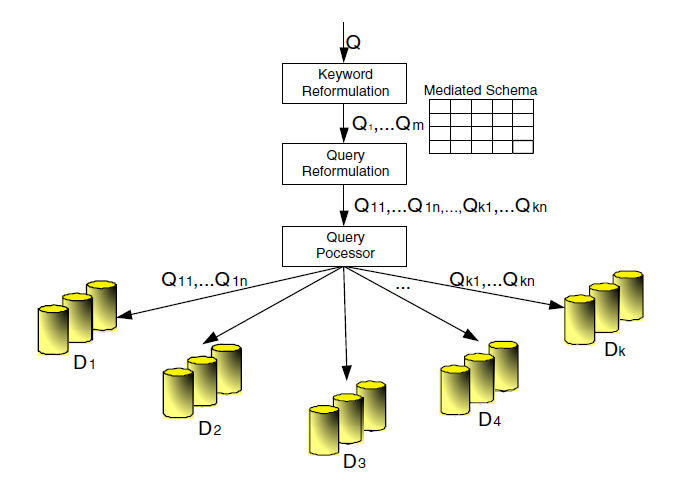
\includegraphics[width=0.75\textwidth]{figures/DataModelingInDSSPs-Figure1.png}
	\end{center}
	\caption{Architecture of a dataspace system that handles uncertainty \cite[p. 124]{DBLP:conf/birthday/SarmaDH09}}
	\label{DataModelingInDSSPsFigure1}
\end{figure}

Different is also the query answering in a DSSP. It doesn't find necessarily all answers on a given query, rather than typically find the top-k answers, and rank these answers most effectively. 
The architecture of the proposed system is shown in \ref{DataModelingInDSSPsFigure1}. The DSSP contains a number of data sources and a mediated schema (probabilistic mediated schemas are omitted here). When the user poses a query, which can be either a structured or a keyword query, the systems returns a set of answer tuples, each with a calculated probability. If a keyword query was posed, a keyword reformulation has firstly be done to translate it into a set of candidate structured queries on the mediated schema. Otherwise, the candidate query is the posed query itself.
\subsection{Probabilistic Mediated Schema Mapping}
\textcolor{red}{\textbf{TODO}}\\
\textcolor{red}{Used Papers: \cite{DasSarma:2008:BPD:1376616.1376702}}

In \cite{DasSarma:2008:BPD:1376616.1376702} was shown, that it is possible to automatically bootstrap a data integration system that answers queries with high precision and recall. In a sense, it is possible to set up a data integration system without any human involvement. With this approach, it isn't possible to answer queries fully accurate and complete as it would be with manual or semi-automatic ones, but best-effort answers and improvement over time are possible by using a probabilistic data model. 
Mediated schemas can be build automatically by clustering attributes from the various source schemas to groups by their semantic meaning and then using this groups as attributes in the mediated schema. Sources in a dataspace typically are heterogeneous, so as a general rule there is more than one possibility to cluster the attributes and it exists an uncertainty of the best(s) grouping(s). If you would choose only one schema of the set of possible mediated schemas, you would likely have a loss in query answering in both terms, precision and recall.  So it seems natural to consider all possible mediated schemas combined in a single mediated schema. By weighting each mediated schema through its likelihood of accuracy, it is possible to favor schemas with a greater weight for query answering and answer ranking. And that is exactly, what a probabilistic mediated schema (p-mediated schema) is doing.
For clustering attributes from the source schemas, similarity functions based on attribute matching are used. Thus, some not very obvious attribute correspondences aren't detected by this approach. But the authors believe, that using more advanced schema matching algorithms like also considering column value similarities, could minimize this problem \cite{DasSarma:2008:BPD:1376616.1376702}.

The concept of probabilistic Schema Mapping (p-mapping) was introduced in \textcolor{red}{Cite!!!}. It describes a probabilistic distribution of possible mappings between a source and a mediated schema. A mathematical formal definition and additional information about probabilistic schema mapping can be found in the original paper \cite{DasSarma:2008:BPD:1376616.1376702}.
 
The whole process is visually represented in \ref{BootstrappingPayAsYouGoDISystems1}, which shows the architecture of the data integration system used by \cite{DasSarma:2008:BPD:1376616.1376702}.

\begin{figure}[H]
	\begin{center}
		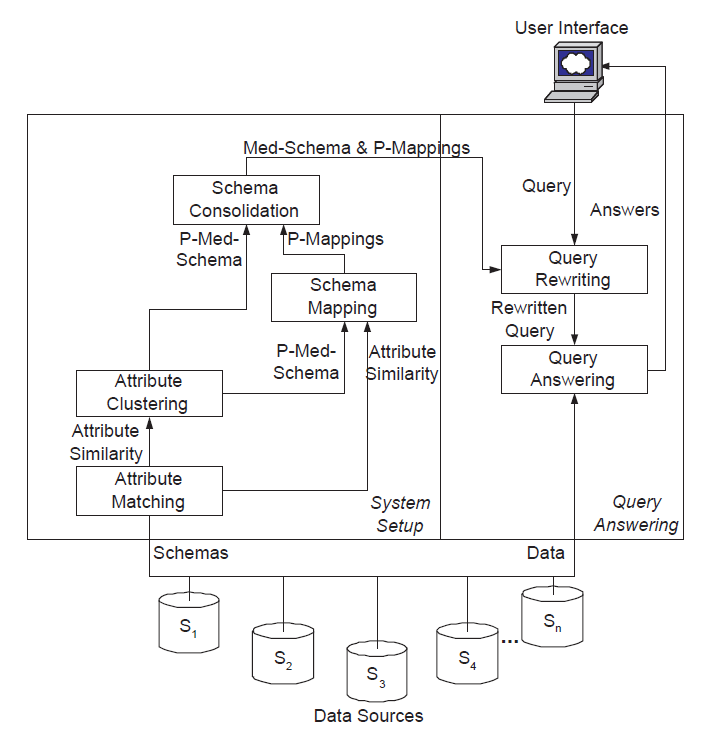
\includegraphics[width=0.75\textwidth]{figures/BootstrappingPayAsYouGoDISystems1.png}
	\end{center}
	\caption{Bootstaping a 'Pay as you go' data integration system}
	\label{BootstrappingPayAsYouGoDISystems1}
\end{figure}

On set-up time, the system automatically generates the p-mediated schema and appertaining p-mappings by clustering the attributes of the source schemas and calculating mapping probabilities afterwards. For the clustering process similarity functions are used, but more advanced techniques could used, as well. After creating the p-mediated schema and its p-mappings, they are consolidated to generate a final mediated schema and p-mappings. Consolidation means to aggregate all possible schemas to one mediated schema and creating p-mappings for this single schema. The purpose of the consolidation is providing the user a sole mediated schema to interact with and additionally it speeds up query answering, as the consolidation process removes redundant information from the p-mediated schema and therefore queries only need to be rewritten and answered based on one mediated schema.
At query-answering time the query is rewritten for each data source according to the mappings and answers the rewritten query on the data sources. Answering queries with respect to p-mappings returns a set of answer tuples, each with a probability indicating the likelihood that the tuple occurs as an answer.

As probabilistic schema mapping is crucial for dataspace systems we want to go a little more in depth by showing a little example of bootstrapping a fictional data integration system providing access to bio-medical information in the field of antimicrobial susceptibility tests:

Let us assume we have 2 data sources S\textsubscript{1} and S\textsubscript{2} . 
Their concepts and data sets are shown in \ref{PMappingExampleConcepts}.

\begin{figure}[H]
	\begin{center}
		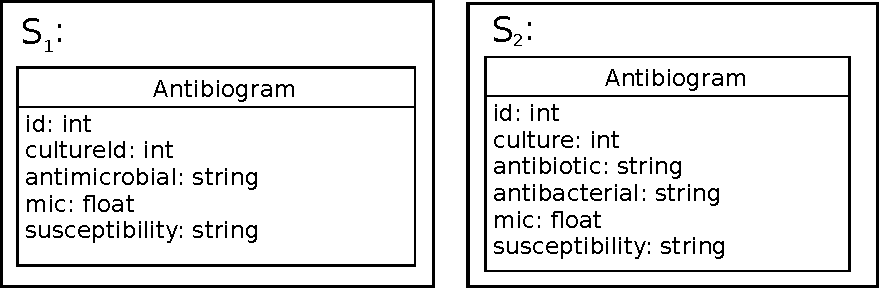
\includegraphics[scale=0.75]{figures/PMappingExampleConcepts.pdf}
	\end{center}
	\caption{Concepts of our example}
	\label{PMappingExampleConcepts}
\end{figure}

Beside syntactic heterogeneity,  the attribute members \textit{antibiotic} and \textit{antibacterial} from S\textsubscript{2} could both possibly matched to \textit{antimicrobial} from S\textsubscript{1}. Clustering using similarity function could thereby result in the following two clusterings (other possibilities are omitted for the sake of simplicity):

M\textsubscript{1}: (\{\textit{id}\}, \{\textit{cultureId}, culture\}, \textit{drug} := \{\textit{antimicrobial}, antibiotic\}, \{antibacterial\}, \{mic\}, \{susceptibility\})\\
M\textsubscript{2}: (\{\textit{id}\}, \{\textit{cultureId}, culture\},  \textit{drug} := \{\textit{antimicrobial}, antibacterial\}, \{antibiotic\}, \{mic\}, \{susceptibility\})

To break it down, the two clusterings show whether \textit{antibiotic} or \textit{antibacterial} are semantically equal to \textit{antimicrobial}. Let us assume that both schemas are equally probable, this means $ P(M\textsubscript{1}) = P(M\textsubscript{2}) =  \frac{1}{2} $.\\
Consequently the p-mediated schema is given by:\\
$M\textsubscript{P}: \{(M\textsubscript{1}, \frac{1}{2}), (M\textsubscript{2}, \frac{1}{2})\}$\\
\raggedright
The appertaining p-mappings are given by \ref{Probabilities-p-mapping} (note, that the probabilities are only for demonstration purposes and weren't calculated):\\
%\begin{table}[]
\centering
\begin{tabular}{|p{0.8\textwidth}|p{0.2\textwidth}|}
\hline
 \textbf{Possible Mapping for M\textsubscript{1}}  &  \textbf{Probability}\\ \hline
 m\textsubscript{11} := \{(id, id), (culture, cultureId), (antibiotic,  \textit{drug}), (antibacterial, antibacterial), (mic, mic), (susceptibility, susceptibility)\}   &  $ \frac{9}{10} $\\ \hline
 m\textsubscript{12} :=  \{(id, id), (culture, cultureId), (antibacterial,  \textit{drug}), (antibiotic, antibacterial), (mic, mic), (susceptibility, susceptibility)\}   &  $ \frac{1}{10} $\\ \hline
\end{tabular}
\begin{tabular}{|p{0.8\textwidth}|p{0.2\textwidth}|}
\hline
 \textbf{Possible Mapping for M\textsubscript{2}}  &  \textbf{Probability}\\ \hline
  m\textsubscript{21} := \{(id, id), (culture, cultureId), (antibacterial,  \textit{drug}), (antibiotic, antibiotic), (mic, mic), (susceptibility, susceptibility)\}   &  $ \frac{8}{10} $\\ \hline
  m\textsubscript{22} := \{(id, id), (culture, cultureId), (antibiotic,  \textit{drug}), (antibacterial, antibiotic), (mic, mic), (susceptibility, susceptibility)\}   &  $ \frac{2}{10} $\\ \hline
\end{tabular}
\captionof{table}{Probabilities of the p-mappings}
\label{Probabilities-p-mapping}
%\end{table}
\raggedright
Now, let's assume, we have the following data set in S\textsubscript{2} containing only one tuple: \{(3180102, 1910181, cefepime, axepim, 0.96, S)\};
And assume we want to process the query:\newline\\

\textbf{Select} drug, mic, susceptibility\\
\textbf{from } Antibiogram\newline\\

Using the schemas M\textsubscript{1} and M\textsubscript{2}, the possible answers would be:
\textit{a\textsubscript{1}} := (cefepime, 0.96, S)\\
\textit{a\textsubscript{2}} :=  (axepim, 0.96, S)\\
\raggedright
To calculate their probabilities and therefore getting the order for a Top-k ranking, we have to consider both, the probability of the schemas and their attending p-mappings. Therefore:\\
$P(a\textsubscript{1}) = P(M\textsubscript{1}) \cdot P(m\textsubscript{11}) + P(M\textsubscript{2}) \cdot P(m\textsubscript{22}) = \frac{1}{2} \cdot \frac{9}{10} + \frac{1}{2} \cdot \frac{2}{10} = \frac{11}{20}$\newline
$P(a\textsubscript{2}) = P(M\textsubscript{1}) \cdot P(m\textsubscript{12}) + P(M\textsubscript{2}) \cdot P(m\textsubscript{21}) = \frac{1}{2} \cdot \frac{1}{10} + \frac{1}{2} \cdot \frac{8}{10} = \frac{9}{20}$\newline
\\
Finally, the top-k answer looks like:\\
{
\centering
\begin{tabular}{|p{0.4\textwidth}|p{0.2\textwidth}|}
\hline
 \textbf{Answer}  &  \textbf{Rank}\\ \hline
  (cefepime, 0.96, S)  &  0.55 \\ \hline
  (axepim, 0.96, S)  &   0.45\\ \hline
 \hline
\end{tabular}
\captionof{table}{Query answer of our example}
\label{query-answer-top-k}
}
%\section{Databases to Dataspaces - A New Abstraction for Information Management}

Dataspaces describes a new abstraction of data management \cite{Franklin:2005:DDN:1107499.1107502}. In current scenarios it is rarely the case, that data to be managed is solely stored in a convenient relational Database Management System (DBMS) or in another, single data model. Therefore, developers often face the challenge to deal with heterogeneous data on a low level base. Challenges are to provide search and query capabilities, enforcing rules, integrity constraints, naming conventions etc.; tracking lineage; providing availability, recovery and access control; and managing evolution of data and meta-data. That issues are ubiquitous and arise in enterprises, government agencies and even on one's PC desktop. 

As a response to this problem, the authors postulate the concept of dataspaces and corresponding to this, the  development of DataSpace Support Platforms (DSSPs). Shortly said, the latter provides an environment of cooperating Services and guaranties, that enables software developers to concentrate on their specific application problem rather than taking care of returning issues in consistency and efficiency of huge, linked but heterogeneous data sets. The remarkable properties of a dataspace system are defined as follows:

A DSSP must deal with data and applications in a variety of file formats, that are accessible through many systems with different interfaces. A DSSP has to support all kinds of data in the dataspace rather than only a few (as DBMSs do).
Although a DSSP provides a integrated possibility for searching, querying, updating and administration, the data often can only be accessible and modifiable through native interfaces. Therefore DSSPs haven't full control over their data.
Queries on a DSSP may offer varying levels of services. In some cases the answers can be approximated resp. best-effort. An example: If some data sources are unavailable for some reasons the DSSP is able to return the best result as possible. Therefore it uses the data that are available at the time of the query.
A DSSP has to provide the tools that allow a tighter data integration process in the dataspace as necessary.

Many of the services a dataspace provide, data integration and exchange systems provide, too. The main difference between these systems is that data integration systems need a semantic integration process before they can provide any services on the data. But dataspace is not kind of a classic data integration approach. In order to avoid semantic integration, a dataspace uses the concept of data coexistence.  The idea is to provide base functionality over all data sources, regardless of their specific integration constraints. E.g. a DSSP is able to provide a keyword search similar to a desktop file search. If more sophisticated operations are required such as relational queries, data mining or monitoring of specific data sources, additional effort can be done to integrate the sources tighter. This incremental process is also called as ``pay-as-you-go'' fashion.

In chapter 3 of the paper the authors pottered at the logical components and services a DSSP should have:

\textbf{Logical components}

A Dataspace should contain all information being relevant for a specific organization/task regardless of their file format or storage location, and it should model a collection of relationships between the data repositories. Therefore the authors define the dataspace as a set of participants and relationships. Participants of a dataspace are individual data sources . Some participants support expressive query languages for querying while others only provide limited access interfaces. Participants can reach from structured, semi-structured right up to unstructured data sources. Some sources provide traditional updates, some are only be appendable, while others are immutable. Further, dataspaces can be nested within each other, which means that a dataspace should be able to be a part of another dataspace.  Thus, a dataspace has to provide methods and rules for accessing its sub dataspaces.

\textbf{Services of dataspaces}

The most basic services a dataspace should contain is the cataloging of data elements of all participants. A catalog is an inventory of data resources containing all important information about every element (source, name, storage location inside the source, size, creation date, owner, etc.)of the dataspace. It is the infrastructure for the most other dataspace services. Search and query are two main services a DSSP must provide. A user should be able to state a search query and iteratively precise it, when appropriate, to a database-style query. For the dataspace approach it is a key tenet that search should be applicable to all of the contents, regardless of their formats.
The search should include both data and meta-data. The user should be enabled to discover relevant data sources and inquire about the completeness, correctness and freshness. A DSSP in fact should be aware of the gaps in its coverage of the domain.  
A DSSP should also support updating data. Of course, the mutability of the relevant data sources determines the effects of updates.  
Other key services would be monitoring, event detection and the support for complex workflows (e.g. it is desired that a calculation is done if new data arrives and that the result will be distributed over a set of data sources). On a similar way a DSSP should support various forms of data mining and analysis. 
Not every participant will provide all necessary interfaces for being able to support all DSSP features. Hence it is necessary, that data sources can be extended on various ways. E.g. a source don't store its own meta-data, so there has to be an external meta-data repository for it. 

\textbf{Components and architecture of a dataspace system}

\uline{Catalog and Browse} Information about all participants and the relationships among them are stored in the catalog. It must also deal with a large variety of sources and supports to provide different levels of information about their structure and capabilities. It is important, that the catalog includes the schema of the source, statistics, rates of change, accuracy, completeness query answering capabilities, ownership, and access and privacy policies for each participant. Relationships may be stored as query transformations, dependency graphs or even textual descriptions. If possible, the catalog should include a basic inventory of the data elements at each participant: identifier, type, creation data and so forth. Then, it can support basic browsing over the participant's inventories.
It isn't a very scalable interface, but it can be used to response to questions about the presence or absence of a data element, or determine which participants have documents of a specific type. 
On top of the catalog, the DSSP should have a model-management environment allowing the creation of new relationships and manipulation of existing ones.

\uline{Search and Query} The component has to offer the following capabilities:

(1) \emph{Query everything:} Any data item should be queryable  by the user regardless of the file format or data model. Keyword queries should be supported, initially. When more information about a participant is collected, it should be possible to gradually support more sophisticated queries. The transition between keyword query, browsing and structured querying should be gracefully. And when answers are given to keyword (or structured) queries, the user should be able to refine the query through additional query interfaces. 

(2)\emph{Structured query:} Queries similar to database ones should be supported on common interfaces (i.e. mediated schemas) that provide access to multiple sources or can be posed on a specific data source (using its own schema). The intention is, that answers will be obtained from other sources (as in peer-data management systems), too. Queries can be posed in a variety of languages (and underlying data models) and should be translated into other data models and schemas as best as possible with the use of exact and approximate semantic mappings.

(3) \emph{Meta-data queries:} It is essential, that the system supports a huge variety of meta-data queries. These include (a) source inclusion of an answer or how it was derived or computed, (b) timesteps provision of the data items that are included in the computation of an answer, (c) specification of whether other data items may depend on on a particular data item and the ability to support hypothetical queries. A hypothetical question would be 'What would change if I removed data item X?. (d) Querying the sources and degree of uncertainty about the answers.
Queries locating data, where the answers are data sources rather than specific data items, should be supported, too. 

(4) \emph{Monitoring:} All stated Search and Query services should also be supported in an incremental form which is also applicable in real-time to streaming or modified data sources. It can be done either as a stateless process, in which data items are considered individually, or as a statefull process. In the latter multiple data items are considered.   

\uline{Local store and index} A DSSP has a store and index component to achieve the following goals:
to create efficiently queryable associations between data items in different participants. Important is here, that the inde should identify information across participants when certain tokens appear in multiple ones (in a sense, a generalization of a join index)
to improve accesses to data items with limited access patterns. Here, the index has to be robust in the face of multiple references to real-world objects, e.g. different ways to refer to a company or person.
to answer certain queries without accessing actual data sources. Thus the query load is reduced on participants which cannot allow ad-hoc external queries. 
to support high availability and recovery

The index has to be highly adaptive to heterogeneous environments. It should take as input any token appearing in the dataspace and return the location at which the token appears and the roles at each occurrence. Occurrences could be a string in a text file, element in file path, a value in a database, element in a schema or tag in a XML file. 

\uline{Discovery Component} This components locates participants in a dataspace, creates relationships between them, and helps administrators to refine and tighten these relationships. For each participant the component should perform an initial classification according to the participant's type and content. The system should provide an environment for semi-automatically creating relationships between existing participants and refining and maintaining existing ones. This involves both finding which pairs of participants are likely to be related, and then proposing relationships which a human can verify and refine. The discovery component should also monitor the content in order to propose additional relationships in the dataspace over time.  
 
\uline{Source Extension Component} Some participants may don't provide significant data management functions. For example, a participant might be no more than departmental document repository, perhaps with no services than weekly backups. A DSSP should support to enrich such a participant with additional capabilities, such as a schema, a catalog, keyword search and update monitoring. It may be necessary to provide these extensions locally as there can be existing applications or workflows that assume the current formats or directory structures.	
This component also supports ``value-added'' - information held by the DSSP, but not present in the initial participants. Such information can include ``lexical crosswalks'' between vocabularies, translation tables for coded values, classifications and ratings of documents, and annotations or linked attached data set or document contents. Such information must be able to span participants in order to link related data items.
%
\textcolor{red}{Following paragraph have to be moved to more suitable place!}\\
The document ``Principles of Dataspace System'' of Alon Haley, Michael Franklin and David Meier\cite{Halevy:2006:PDS:1142351.1142352} is based on their previous work ``From Databases to Dataspaces - A New Abstraction for Information Management''\cite{Franklin:2005:DDN:1107499.1107502} where the concept of dataspaces was firstly presented, and poses specific technical challenges realizing Dataspace Support Platforms (DSSPs) relating to query answering, introspection and the benefits of human attention for improving semantic relationships within a dataspace.  
In the following are stated the results of the above mentioned challenges:


\subsection{Query answering}

Queries are posed in a wide range of different languages. Most of the activities will properly begin with a keyword search, but it will also be common to see queries as a result of a form (which results to queries with several selectable predicates). It will come to more complex queries when a user interacts deeper with a certain data source. If it isn't explicitly stated, it is usual, that a user is likely to believe that a query considers all relevant data in a dataspace, regardless of the used data model or schema. Even if a query is posed to a data source, it is implicitly expected that the system considers the data of other sources, as well. If additional answers are desired, one has to do transformations on the schema and the data model.

\textbf{Challenges of answer querying}

Answers corresponded to queries of a dataspace are different from traditional queries in several ways. The challenges to it are analyzed more deeply in the third chapter:

\uline{Ranking:} Queries are typically sorted by their relevance, similar to a web search engine. Ranking is necessary not only for keyword search, but also for structured queries, when transitions to other data sources should be approximated.  

\uline{Heterogenity:} Answers will come from many sources and will differ in their used data model and schema. The Ranking has to manage heterogeneity, too.

\uline{Sources as answers:} In addition to base elements (e.g. documents or tuples), a DSSP should be able to provide sources, as well. This means that it returns links to locations where additional answers can be found.

\uline{Iterative queries:} Normally, the interaction with a dataspace can't be reduced to the process of posing  a sole query and getting an answer to it. Instead, a user is involved in an information finding task that requires a sequence of queries, each being a refinement or modification on the previous ones.

\uline{Reflection:} It is expected, that a DSSP reflects on the completeness of its coverage and the accuracy of its answers. 


\textbf{Dealing with challenges}

The first step to face these challenges is to build a formal model. Therefore, the authors propose five directives:

\uline{Challenge 3.1.}  The development of a formal model for analyzing the query answering in a dataspace. 

\uline{Sub-Challenge 3.2.} The development of intuitive semantics to answer a query taking into consideration a sequence of earlier posed queries. 

\uline{Sub-Challenge 3.3.} The development of a model for an information finding task which includes operations on lower levels. 

\uline{Sub-Challenge 3.4.} The development of algorithms sorting the data sources according to how likely they are to contain the answer. These algorithms should start from a keyword query and operate on a large collection of data sources.

\uline{Sub-Challenge 3.5.} The development of methods for ranking answers retrieved by multiply heterogeneous data sources.


\textbf{Query answering model and challenges}

\uline{Challenge 3.7.} The development of techniques to answer queries based on the following ideas or  
combinations of it:

- apply several approximate or uncertain mappings and compare the answers obtained by each.

- apply keyword search techniques to obtain some data or some constants that can be used in instantiating mappings.

- examine previous queries and answers obtained from data sources in the dataspace and try to infer mappings between the data sources. Whenever we have access to queries that span multiple data sources, try to infer from them how the sources are related (e.g., the join attributes should provide some hint of common domains).

- Develop a formal model  for approximating semantic mappings and for measuring the accuracy of answers obtained with them.

- Develop automatic best-effort methods for translating a query over one data set onto the other.

\textbf{Introspection}

In chapter 4 introspection within a dataspace is analyzed. Introspection describes on this occasion the ability of a dataspace to observe assumptions and uncertainties and specifying their origin. In contrast to traditional databases introspection isn't a nice feature but a necessity. Introspection has to be possible over the following highly related parameters: Lineage, Uncertainty and Inconsistency. Thus, one speaks of LUI introspection in the context of dataspaces.

\textbf{Uncertain databases }

Uncertainty arises in applications for data management if the exact state of the (data) world is not known. The goal of a uncertain database is to represent a set of possible states the world can have. Usually, the states are referred to as possible worlds. Every possible world represents a complete valid state of the database. For declaring these states there were developed several formalisms \cite{FoundationOfDatabases1995, Barbara:1992:MPD:627288.627535, WorkingModelsForUncertainData, Grahne:1984:DSD:645912.671297, Lakshmanan:1997:PFP:261124.261131}. Examples for formalisms would be a-tuples, x-tuples or c-tables\cite{DBLP:reference/db/Grahne09a}.


\textbf{Inconsistency in databases}

The task of an inconsistency database is to handle situations where the database contains conflicting data. A common example would be the existence of two values of a salary of an employee whereby the values are obtained from different data sources. The essence for solving this problem is to consider all possible repairs. A repair is a minimal change resulting the database to a consistent state. As a rule, there are more one one possibility which is why the database owns several repairs to choose from. That's also the reason for the tight relationship between uncertainty and inconsistency as inconsistency can be interpreted as uncertainty over the knowledge, which of the conflicting value is the best solution.

\textbf{Modeling of data lineage}

The lineage of a tuple reports how the tuple was derived from a certain data set. There is a distinction to internal and external lineage. Internal lineage applies to tuples of a query result -- lineage specifies here how the tuple was derived within a database. External lineage relates to tuples inserted into a database, the lineage relates hereby to the external sources or processes by which the tuples were inserted. 

\textbf{LUI Introspection}

A DSSP should provide a uniform mechanism for modeling uncertainty, inconsistency and lineage. Thereby the following challenges arise:

\uline{Challenge 4.1.}  Develop a formalism for enabling the modeling of uncertainty, inconsistency and lineage.

\uline{Sub-Challenge 4.2.}  Develop a formalism which captures the uncertainty over general forms of inconsistency in databases.

As inconsistency results to a special type of uncertainty, the formalism for uncertainty should leverage this special structure. The formalism for uncertainty tells us only what the possible states of the world are and sometimes it assigns every possible world its corresponding possibility. But in many cases, it is the only way to resolve uncertainty and to get knowledge about data lineage and how and where the data was derived from.

Web search engines already unify uncertainty and lineage in a simple way. One of the main reasons why the authors want to unify lineage and uncertainty is to reason the relationship between external sources and their impact on answers. Thereby arises the following challenges:

\uline{Sub-Challenge 4.3.}  Develop a formalism which represents the external lineage and reasons it.

To combine uncertainty and lineage, there exists

\uline{Sub-Challenge 4.4.}  Develop a general technique for extending every kind of uncertainty and for investigating the representative and calculative advantages of this procedure. 

To achieve this, the object that should be assigned uncertainty, has to match to the object lineage is attributed to. 

\textbf{Uncertainty on Views}

There's a general problem with modeling uncertainty as the uncertainty formalism associate uncertainty with a single schematic construct: tuples in the case of x-tuples and attribute values in the case of a-tuples. So the chose of database schema and normalization limits the kinds of uncertainty to express. In the case of using views, the authors propose to link uncertainty with the view's tuples, hence:

\uline{Sub-Problem 4.5.} Develop formalisms where uncertainty can be attached to tuples in views and view uncertainty can be used to derive uncertainty of other tuples

\textbf{Finding the right answer}

This chapter address to what has to be done to determine the quality of a query answer (how good is a query?).

\uline{Sub-Challenge 4.6.} Define metrics for comparing the quality of query answers and answer sets over a dataspace, and find efficient techniques to process queries.

A limited version of this issue was already addressed with minimal repairs related to inconsistent databases. Here it will be tried to construct a consistent database as tight as possible on the base of the inconsistent one. For improving the results, it is necessary to do some preferences, which results in the following challenges:

\uline{Sub-Challenge 4.7.} Develop query-language extensions and their corresponding semantics that enable specifying preferences on answer sets along the dimensions of completeness and precision, certainty and inconsistency, lineage preferences and latency.

Along with the specification of preferences there are needed methods for reasoning query answer sets. This is essential for comparing answer sets. Query containment \cite{Chandra:1977:OIC:800105.803397} will be extended in the context to dataspaces. By which the following challenge submits to:

\uline{Sub-Challenge 4.8.} Define notions of query containment that take into consideration completeness and precision, uncertainty and inconsistency and lineage of answers, and efficient algorithms for computing containment.

The following issues stands in relation to section 4.1. of the paper:

\uline{Sub-Challenge 4.9.} Develop methods for efficient processing of queries over uncertain and inconsistent data that conserve the external and internal lineage of the answers. Study whether existing query processors can be leveraged for this goal.

%\subsection{Towards Realization of Dataspaces}

In the paper ``Towards Realization of Dataspaces'', written by Ibrahim Elsayed and Peter Brezany\cite{1698348}, the architecture and functionality of a Dataspace Management System(DMS) is presented. Additionally it is discussed, how grid technology of future implementations is able to support such an architecture. A DMS is a set of software programs, which controls the organization, storage and retrieval of data in a Dataspace. It also handles the security and integrity of a Dataspace.
In the following, the architecture and the functionality requirements of a DMS will be described.   

\textbf{{\large Requirements}}

\begin{figure}[H]
	\begin{center}
		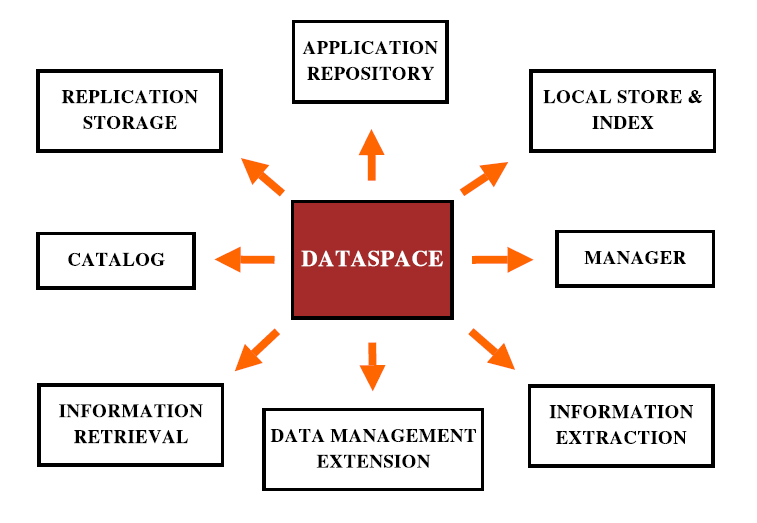
\includegraphics[width=0.75\textwidth]{figures/TowardsRealizationOfDataspaces1.png}
	\end{center}
	\caption{Environment of  a Dataspace}
	\label{TowardsRealizationOfDataspacesEnvironment}
\end{figure}

\uline{Information Retrieval:} Queries and searches are two different methods of information retrieval and represent together one of the main services a DMS should support. Generally, queries and searches should be supported by all participants of the Dataspace, regardless of their used data model. It shouldn't make a difference for a user to operate on a sole database or on a Dataspace. A good known and simple search operation is keyword searching. The Support of spanning such a search method over all participants, is a challenging research topic. The development of methods for keyword searching on relational and XML databases was done by the data-engineering community \cite{994693, Guo:2003:XRK:872757.872762, Hristidis:2002:DKS:1287369.1287427}, For supporting a global query functionality allowing to formulate uniform queries on all Dataspace participants, intelligent methods for interpreting and translating of queries in several languages are required. Methods for query translation were investigated by a large body of research communities \cite{Carey00xperanto:publishing, 1319983}. 

\uline{Information Extraction:} The world-wide web has become a large data container, by now. For allowing to postprocess data obtained from the web, techniques for web information extraction, extracting relevant information from semi-structured web pages should be supported. For further processing, extracted content has to be converted to structured data and saved locally. Non structured web documents have to be classified first using text mining techniques, which organize the parsed documents into groups with the help of ontologies \cite{conf/wise/HeQZW04}. Based on these ontologies, a keyword search is possible to find individual documents. Structured documents allow easier access and integration due to the rich semantically information included in the data representation.\\
\uline{Data Management Extensions:} This component provides possibilities to improve low-level working Dataspace components. All these base components have only limited data management capabilities. It is a task of a DMS to provide additional functionality such as backup, recovery and replication.\\
\uline{Catalog:} Contains a detailed description of all participants of the Dataspace. Beside basic information about the participants, such as owner, creation date, etc., the description for each participant should also contain semantic information about its data. A user should be able to browse the catalog for getting more detailed information about certain data sources. The catalog may reference a meta-data repository to separate the basic and more detailed descriptions.\\
\uline{Manager:} In order to realize the above mentioned functionality, a central component managing the system and interacting with the user is needed. Alongside user authentication, right assignments and other services, this manager component is responsible for communicating with all participants. Thus, this component serves as an interface between the users and the participants of the Dataspace.\\
\uline{Local Store and Index:} This component is responsible for caching search and query results, so that certain queries can be answered without the need of accessing the actual data sources. Furthermore it supports the creation of queryable associations between the participants.\\
\uline{Replication Storage:} Allows to copy participant data in order to increase its access time. This results in high availability and high recovery is supported.\\
\uline{Application Repository:} With this component, the user is able to share data analysis tools, domain specific models, evaluations, etc., which can be applied to the (available) data of the Dataspace.\\
\begin{figure}[H]
	\begin{center}
		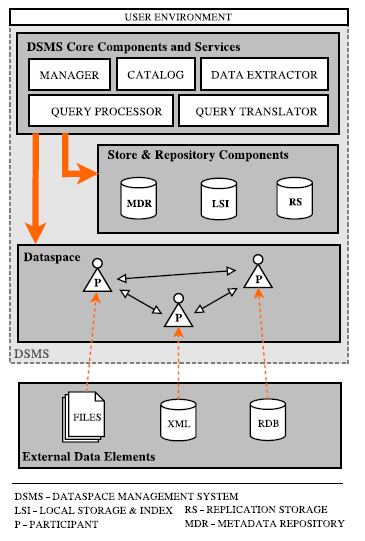
\includegraphics[width=0.75\textwidth]{figures/TowardsRealizationOfDataspaces2.png}
	\end{center}
	\caption{System architecture}
	\label{TowardsRealizationOfDataspacesArchitecture}
\end{figure}
Generallly, a Dataspace consists of Dataspace components, the so-called participants, and relationships between the participants. Components are individual data sources, such as relational databases, text databases, XML databases, data stream systems, web services or other data archives.\\
A Dataspace component includes a description for describing what data it contains, which storage formats are used and which query mechanisms are supported. In addition it contains information about the storage location of the data and whether the data was replicated, equally it contains information about relationships to other participants. The information and data are marked if they are added by the management system, the user or were automatically generated.  \\
Each participant is described the same way as the components and is subsequently registered within the catalog. Thus they are available as data sources for a more abstracted layer, which provides global query and search methods. This global layer is embedded in the DMS. It supports the user to create new Dataspace components, to add relationships between other participants, to register participants within the catalog, to browse the catalog for available participants, to decide whether to share all or only  selected participants within a community including assignments of rights, and to search all or only selected participants of a Dataspace.\\
As each participants is managed by its own and thus is responsible for its data management such as data update, recovery and replica, it isn't a task of the DMS to change the data represented by the participants. Therefore, the DMS has no administration privileges for writing and changing content of the data of a participant. But the DMS provides possibilities to add missing data management services, such as data replication, transformation, download, upload, etc.. 

\textbf{Managing Sub-Dataspaces}\\
The idea behind a Sub-Dataspace is to create a new Dataspace that is included by a another and thus is a subset of a  bigger Dataspace. This functionality is needed for access privileges and security management. An administrator of a Dataspace is thus able to define different data access rights for certain groups.  

%\section{Data Modeling in Dataspace Support Systems}

In the paper ``Data Modeling in Dataspace Support Systems'' \cite{DBLP:conf/birthday/SarmaDH09}, the authors face the issue of uncertainty in dataspaces. In their view, a dataspace needs to model uncertainty in its core. In their work, they described the concepts of probabilistic mediated schemas and probabilistic mappings as enabling concepts for DSSPs. With this foundation, it is possible to completely bootstrap a pay-as-you-go integration system.

Current data integration systems are essentially a natural extension of traditional databases in that queries are specified in a structured form and data is modeled in one of the traditional data models like relational or XML. The System for data integration also has exact information about how the data in the sources map to the schema used for integration. So, for data integration there is a need for large upfront effort in creating the mediated schema and the schema mappings. Dataspace Support Platforms (DSSP) shall considerable reduce this upfront effort. The system should be able to bootstrap itself and provide useful services with no human intervention. When the data management needs become clearer (through user feedback or as sources are added), the system evolves in a pay-as-you-go fashion. 
In order to develop DSSPs, it is impossible to rely on the same data modeling paradigms data integration systems use. One cannot assume, that the mediated schema is given in advance and that the schema mappings between the sources and the mediated schema will be accurate. Therefore the authors argue that uncertainty has to be considered in the mediated schema and in the schema mappings.

\subsection{Uncertainty in Data integration}

\textbf{Sources of Uncertainty}

\uline{Uncertain mediated schema:} The set of schema terms in which queries are posed is called the mediated schema. Not necessarily they cover all the attributes in any source, it cover rather the aspects of the domain that the developer of the application wishes to expose to the user. For several reasons uncertainty happens in the mediated schema. First, if the mediated schema is derived from the data sources during bootstrapping, there will be some uncertainty about the results. When domains are broad, there will be also some uncertainty about how to model them, because in general, there will be overlappings in different topics. 

\uline{Uncertain schema mapping:} Schema mapping defines the semantic relationships between the terms in the sources and the terms used in the mediated schema. Although, schema mappings can be inaccurate. In a dataspace, many of the initial schema mappings are properly automatically derived, and therefore they may inaccurate. In general, it is impossible to create and maintain precise mappings between data sources. 

\uline{Uncertain data:} Some of the data may be obtained by automatisms as data sources may not always be structured well. Additionally, unreliable or inconsistent data may be contained in systems with many sources. 

\uline{Uncertain queries:} Properly, much of the early interaction with a dataspace will be done through keyword queries as the users aren't aware of a (non-existent) schema. The queries have to be translated into some structured form so they can be reformulated with respect to the data sources. At this point, multiple candidate structured queries could be generated and thus some uncertainty arises about which query captures the real intention of the user.

\subsection{System architecture}

The most fundamental characteristic of this system is that it is based on a probabilistic data model. In contrast to a traditional data integration system, which includes a single mediated schema and assumes a single (and correct) schema mapping between the mediated schema and each source, the data integration module of a DSSP attaches possibilities to multiple tuples, mediated schemas, schema mappings and possible interpretations of  keyword queries posed to the system. 

For DMS it is assumed that queries are posed as keywords. This is contrary to traditional integration systems which assume the query to be posed in a structured fashion( i.e. that it can be translated to some subset of SQL). So, a DSSP must first reformulate a keyword query into a set of candidate structured queries, before it can reformulate the query onto the schemas of the data sources. This step is also called keyword reformulation.  It is important to note, that keyword reformulation differs from keyword search techniques on structured data (see \cite{994693}, \cite{Hristidis:2002:DKS:1287369.1287427}) in that (a) it does not assume access to all data in the sources or that the sources support keyword search, and (b) it tries to distinguish different structural elements in the query in order to pose more precise queries to the sources. In any case, keyword reformulation should benefit from techniques that support answering search on structured data.

\begin{figure}[H]
	\begin{center}
		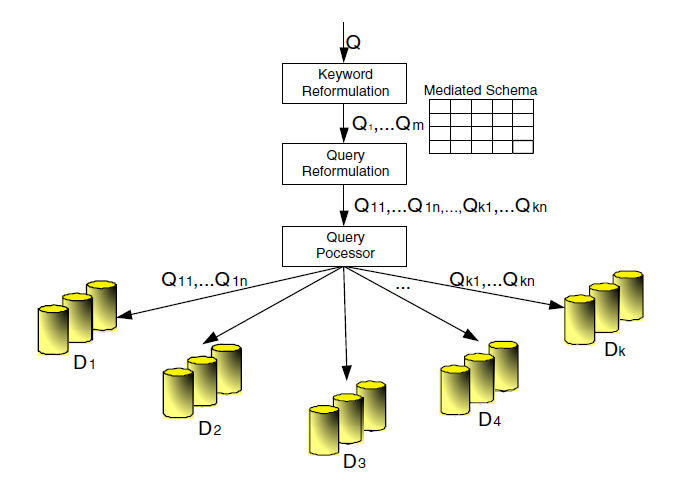
\includegraphics[width=0.75\textwidth]{figures/DataModelingInDSSPs-Figure1.png}
	\end{center}
	\caption{Architecture of a data integration system that handles uncertainty}
	\label{DataModelingInDSSPsFigure1}
\end{figure}

Different is also the query answering in a DSSP. It doesn't find necessarily all answers on a given query, rather than typically find the top-k answers, and rank these answers most effectively. 
The architecture of the proposed system is shown in \ref{DataModelingInDSSPsFigure1}. The DSSP contains a number of data sources and a mediated schema (probabilistic mediated schemas are omitted here). When the user poses a query, which can be either a structured or a keyword query, the systems returns a set of answer tuples, each with a calculated probability. If a keyword query was posed, a keyword reformulation has firstly be done to translate it into a set of candidate structured queries on the mediated schema. Otherwise, the candidate query is the posed query itself.
\section{Towards a Model for Multimedia Dataspaces}

In the paper 'Towards a Model for Multimedia Dataspaces'\cite{6167826} the authors present a representation model for dataspaces, which is an approach based on the dataspace and dataspace-view paradigm for uniformly represent  structured and semi structured data, ontologies and other similar knowledge representation models. 
With that model, the authors address the current explosion of digital information and data sources. Many branches (i.a. in the medicine) need now large amounts of distributed, heterogeneous data. 

However, traditional data integration methods are barely applicable to formulate search queries on a distributed,  heterogeneous data set, containing files with many different file formats, as traditional data integration systems are designed for complete structured data.
Thus, these systems need a global schema for calculating search queries. 
Addressing this issue, the concept of dataspaces was developed as an abstraction of wide-area, heterogeneous and distributed data management.
For dataspaces there is no need of upfront efforts to semantically integrate data before basic services such as keyword search can be provided. 

Dataspaces support uncertainties in schema-mapping and consider that schema mapping from sources to  mediated schema may be incorrect.
A further interesting feature of dataspaces is successive data integration. So, the system is able to  integrate data in iterations as the time goes on depending on user needs.

Research in the field of dataspaces is currently very active, but despite of the deep interest, existing models suffer on a number of shortcomings limiting their applicability.
These include the tendency of overlooking the different types of relations that can exist between data items, which restricts the amount of information they can generally integrate.
Second, they focus on classical text data ignoring the specifics of multimedia data. Third they don't provide the fine-granularity in the persistence of integrated data that is needed in certain domains.

To address these issues, the authors developed a dataspace model, which sees the dataspace as a set of classes, objects (instances of classes) and relations.
In the latter case there exist relations between classes (CRC), relations between objects and classes (ORC) and relations between objects (ORO).
Furthermore relations can be internal or external defining whether the anticipating relation objects are in the same data source or in different ones.

A design goal of the model is the maximization of its expression in terms of the types of relations that it can represent, enabling it to deal with information originating from structured data, semi-structured data, ontologies and other forms of knowledge representation as well as from canonical  
knowledge.

Import to note is the fact that the model includes similarity relations in the type of relations. 
Similarity functions are a feature of multimedia data that defines a measurement for non-exact matching between objects.
This kind of relations can be used to derive relations between other objects in the dataspace.
Additionally the model introduces the concept of dataspace-view. 
This makes it possible to store query results of an existing dataspace into a new sub-dataspace with different modes of persistence(virtualized view, materialized view, mode of synchronization with the content of the original sources,...).\\
\chapter{Reference Projects}

In this chapter we will analyze related data integration and dataspace works in the healthcare sector. This will help us to properly design and implement our own system.

We will cover the following works:

\begin{itemize}
\item DebugIT which has a mediator-based architecture and uses ontology-based data integration.
\item 'Dataspace Integration in the medical research' the doctor thesis of Sebastian H.R. Wurst
\end{itemize}

\section{DebugIT}
The DebugIT project is a good reference for analyzing how medical data integration can be done though this project didn't use a dataspace approach but an ontology-mediated \cite{WurstDiss, DBLP:books/dp/LeserN2006} approach. DebugIT stands for ``Detecting and Eleminating Bacteria Using Information Technology'' and its main goal is to provide a platform for high-throughput analysis of distributed clinical data as a response to the spread of antibiotic resistance of infectious pathogens in European hospitals\cite{UniFreiburgDebugITInfo}. 
The team of the DebugIT project released the architecture of their system in \cite{DBLP:conf/swat4ls/SchoberCDEDJTPLB14}.
In that paper it is stated, that the system uses an ontology-based approach for allowing antibiotics resistance data being semantically and geographically interoperable. This makes it possible to integrate distributed clinical data EU-wide in real-time for monitoring antibiotic resistance. As well, the system is structured in four tiers and works in a service oriented manner (SOA). Figure \ref{DebugITArchitectureFigure} shows the layered architecture of the system of DebugIT.

\begin{figure}[]
	\begin{center}
		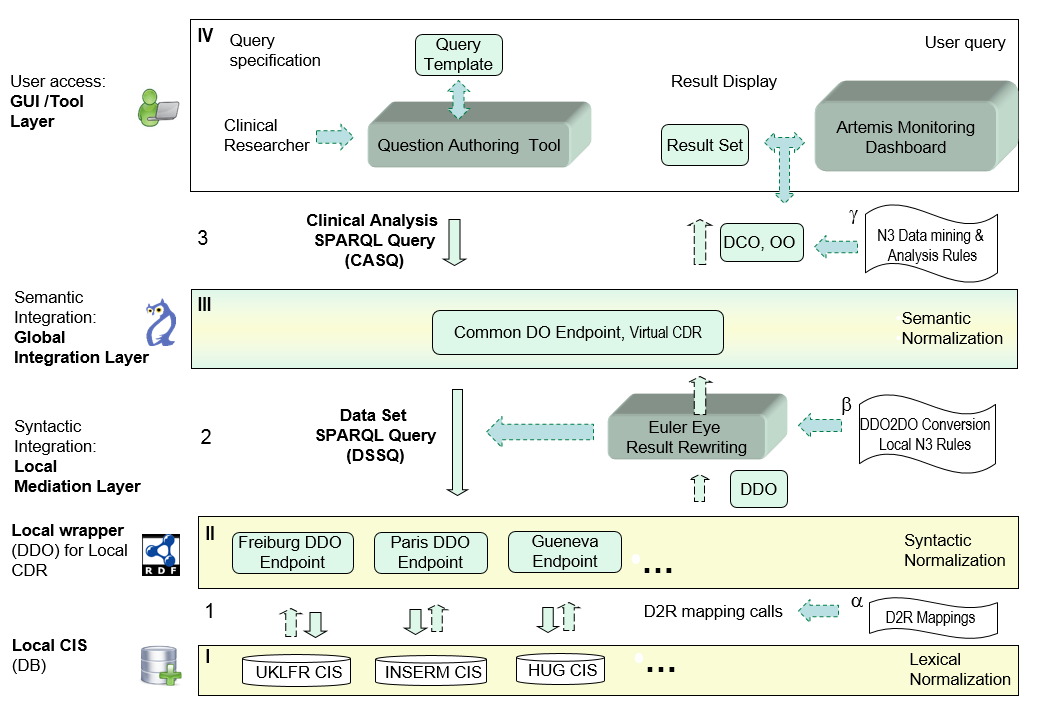
\includegraphics[width=0.75\textwidth]{figures/DebugIT-Ontology-mediated-layered-Data-Integration-architecture.png}
	\end{center}
	\caption{The layered mediator architecture of the DebugIT project}
	\label{DebugITArchitectureFigure}
\end{figure}

Altogether there are 3 data representation layers marked with the Roman Numerals I-III. The query flow between the data layers is specified with 1-3 and the corresponding mappings are given with the Greek letters \textalpha , \textbeta,  and \textgamma .

On the first integration layer (\textbf{I}) relational data are lexical normalized by the use of mappings of medical terminology and morphosemantic mapping employed by the Averbis Morphosaurus software\cite{DaumkeDiss}. Ambiguities can be resolved with ontological expressions (formulated in OWL) on the integration layers II and III. 

The layer \textbf{II} works with RDF data, wherefore relational data from the layer I is transformed to RDF through D2R mapping calls \footnote{http://d2rq.org/} on the\emph{ first mediation layer} (1). On the second integration layer information about the data and their corresponding vocabulary is stored in Data Definition Ontologies (DDOs) \cite{DebugITDDO}. A DDO bridges a local data model and a semi-formal data model on the local mediation layer for integrating syntactic data and provides an Extract, Transform, Load (ETL)-process \footnote{DBLP:books/dp/LeserN2006} for the next integration layer. So materialized data integration is partially done on this layer.
For each Clinical Data Repository (CDR) such a DDO is locally created. A CDR contains clinical data of a specific hospital, institute or is a compound of CDRs.
Layer II contains also a SPARQL endpoint, for allowing Layer III to query its data. These queries are specified through a Data Set SPARQL Query (DSSQ). 

On the \emph{second mediation layer} (2), in the figure called local mediation layer, the local DDO data is bind to the global DebugIT Core Ontology (DCO) \cite{Schober_developingdco:}, which s the ontology of layer III. The corresponding mapping is done through DDO2DCO using the N3 language \footnote{http://www.w3.org/TeamSubmission/n3/} and Simple Knowledge Organization Structure (SKOS) mappings \footnote{http://www.w3.org/TR/2009/REC-skos-reference-20090818/}. The schema mapping is done by the Euler Eye Reasoner \footnote{http://eulersharp.sourceforge.net/}, which also creates implicit knowledge using logical inference.

Data layer \textbf{III} represents a virtual Clinical Data Repository (vCDR), which joins the local Clinical Information Systems (CISs). Important to know is, that in the vCDR are now fully (semantically) integrated and as the name implies, a vCDR \emph{virtually} integrates the data. So data is not duplicated anymore. Through the virtualisation, data of all CIS can be globally queried. Also privacy issues can properly be handled, as the data is not stored outside from the CISs.
Also on layer III clinical analyses can be performed over Clinical Analysis SPARQL Queries (CASQ (3)). 

On the last layer (\textbf{IV}), a user or a monitoring tool can query the integrated clinical data.

Summarizing it, the mapping is performed iteratively in a stack-like manner:
The first mapping \textalpha (D2R mappings) transforms the relational database layer (I) to the RDF representation layer (II). The next mapping \textbeta (N3 and SKOS) transforms the RDF layer II to the Domain Ontology (OO) layer III, where the data is globally queryable as CASQ over mapping \textgamma (DCO and OO).  

\section{Dataspace Integration in the medical research}

'Dataspace Integration in the medical research' (original title 'Dataspace Integration in der medizinischen Forschung') is a german doctor thesis, was written by Sebastian H.R. Wurst and submitted in 2010 \cite{WurstDiss}.

\begin{figure}[H]
	\begin{center}
		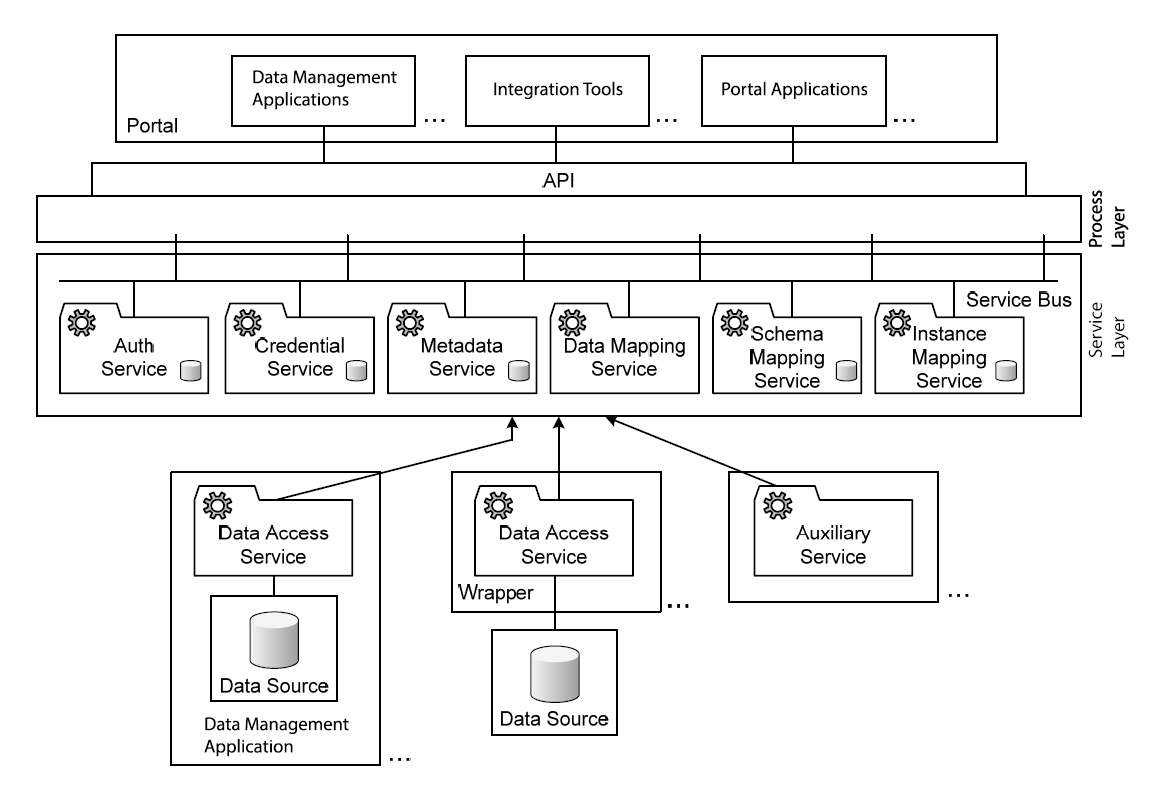
\includegraphics[width=0.9\textwidth]{figures/DataspaceIntegrationInDerMedForschungFigure31.PNG}
	\end{center}
	\caption{Overview of the software architecture of the system used in the doctor thesis of Sebastian H.R. Wurst \cite[p. 117, Figure 31]{WurstDiss}}
	\label{DebugITArchitectureFigure}
\end{figure}
\chapter{MeDSpace}

In this chapter we will present the developed system MeDSpace (\textit{abbr.} for Medical Dataspace) whereas in the next chapter we will look at more implementation specific details.

The purpose of MeDSpace is to provide a distributed test environment of medical datasources. The focus thereby is the provision of a keyword search functionality over medical datasources. 
As distributed keyword search is the foundation for every Dataspace system, MeDSpace can be used as a starting point for a much more evolved dataspace or as a framework for implementing advanced dataspace functionality.
Although the system uses medical datasources for its test data, the system is general enough to be used for other dataspace-related projects or systems, that need keyword search functionality over a set of multiple heterogenous (multimedia) datasources. 

In figure \ref{MeDSpaceOverview} the overview of the MeDSpace system is illustrated.
\begin{figure}[H]
	\begin{center}
	%\hspace*{-1cm}
		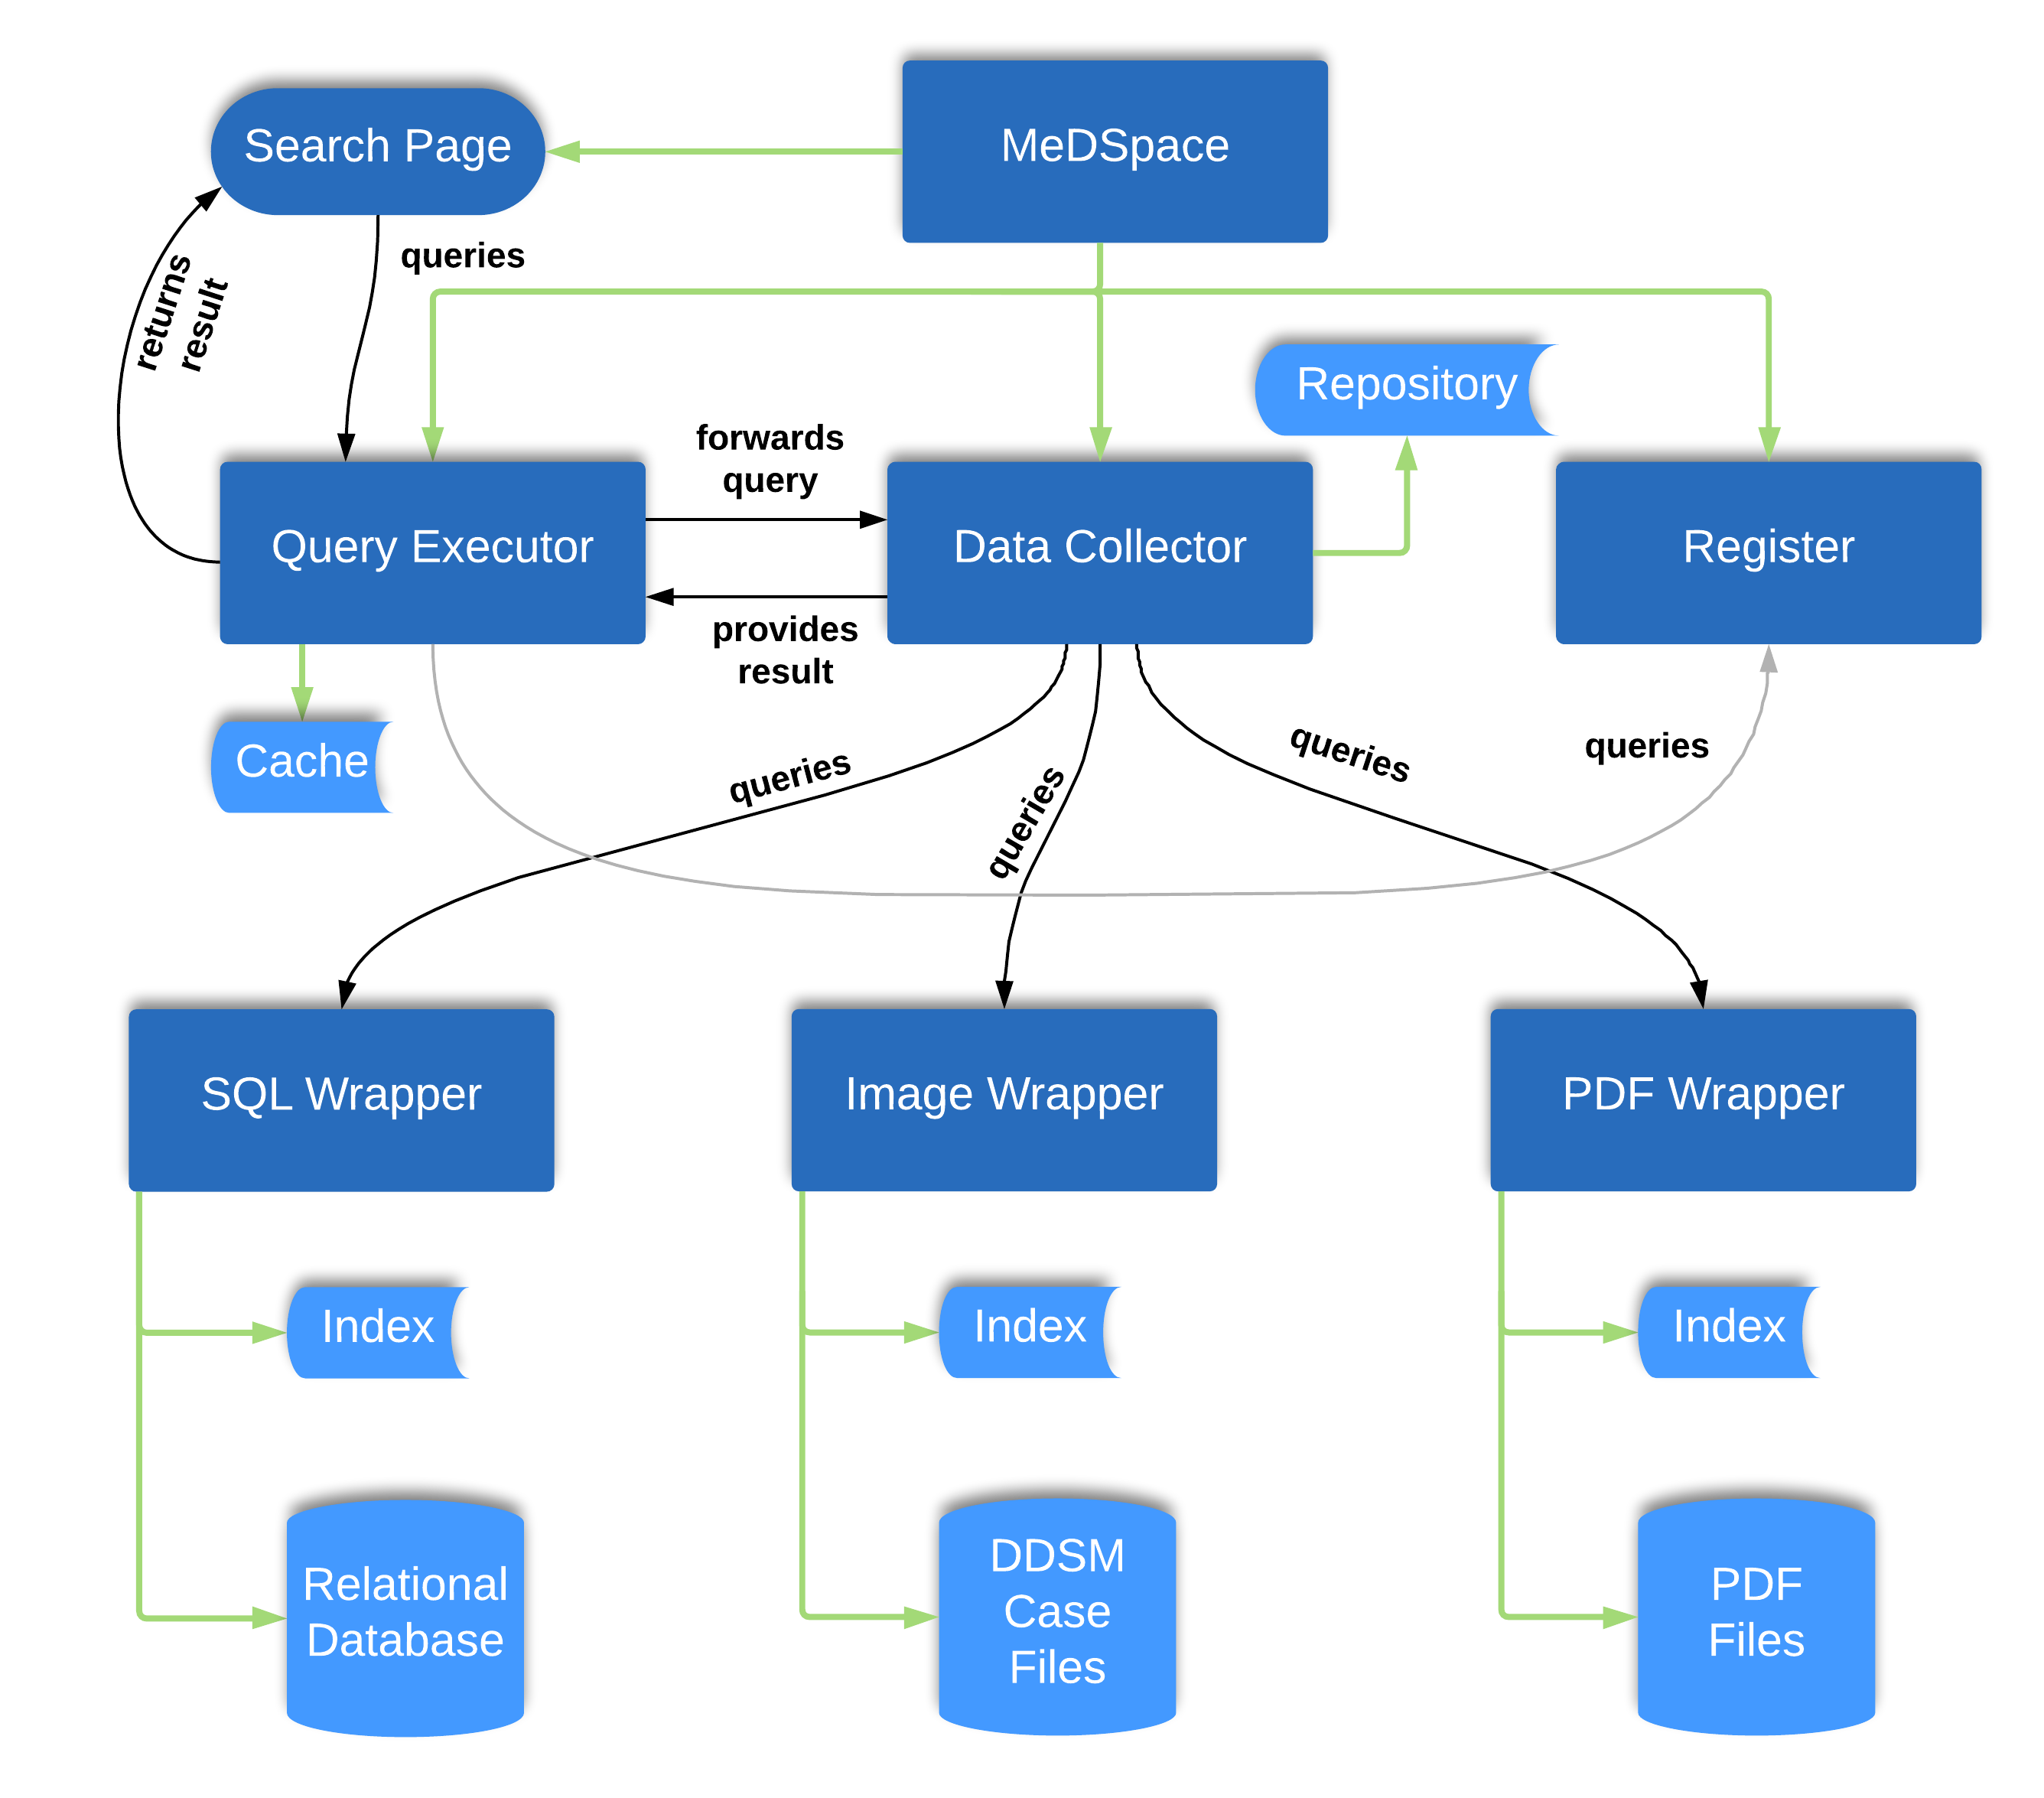
\includegraphics[scale=0.145]{figures/MeDSpace-Overview.png}
	\end{center}
	\caption{MeDSpace Project overview}
	\label{MeDSpaceOverview}
\end{figure} 

The system can roughly be divided into a \emph{wrapper} and a \emph{global MeDSpace} category: The \emph{wrapper} category includes everything from managing the data of a specific datasources (e.g. from a relational database). 
Whereas the \emph{global MeDSpace} category comprises datasource management and services on a global view.  The modules belonging to this category are the \emph{Register}, the \emph{Data Collector}, the \emph{Query Executor}, and the \emph{Search Page}.  

Now, we want look at the requirements met by MeDSpace. Therefore we look at the purposes of each module of the system. 

\section{Wrappers}
Each local datasource has its own wrapper. The wrapper is similar to the wrappers used in a mediator-based system, but provides dataspace specific functionality: the wrapper...
\begin{itemize}
	\item manages the data exchange between the datasource and extern MeDSpace services.
	\item provides keyword search functionality (if the datasource doesn't provide itself). Therefore it creates an index of the data of the wrapped datasource and maintains it. 	
	\item converts search results from the datasource to the canonical data model.
	\item registers and deregisters the datasource from MeDSpace by communicating with the \emph{Register} module. The wrapper informs the register what services the datasource and the wrapper provide.
	\item overcomes technical, syntactic and data model heterogeneity. 
\end{itemize}

Thereby the \emph{SQL Wrapper} is responsible for wrapping a relational database containg data created with the \emph{Patient Data Generation Framework} (PDGF) tool created by Schmiedbauer \cite{SchmidbauerBachelorThesis}. The \emph{Image Wrapper} provides access to case files of \emph{Digital Database for Screening Mammography} (DDSM)\cite{DDSM} and the \emph{PDF Wrapper} maintains a set of pdf files that were created specific for this system: the pdf files contain data based on Schmidbauer's test data.

\section{Register}
The Register holds a list of active datasources that can be queried. Therefore it provides functionality so that wrappers can register and deregister a datasource. In order to know what services are provided by each datasource, the register also keeps records of these services. This allows other modules to use services of any datasource.
\section{Query Executor}
The task of the \emph{Query Executor} is to accept a given keyword search query, transform this query to a service call and instructs the \emph{Data Collector} module to call the keyword search service for each registered data sources. To know which datasources are registered, this module communicates with the \emph{Register} module. After the \emph{Data Collector} has collected the query results of all datasources the \emph{Query Executor} adds the search query to its query cache and returns the collected search result to the caller who requested the \emph{Query Executor}. On the next request, the cached query result will be returned without querying the datasources if no 'cache miss' has been occurred.

Note: It is not the task of the \emph{Query Executor} to actually collect the search result from the datasources. That is done by the \emph{Data Collector}. It does only instruct the \emph{Data Collector} to do the collecting.

\section{Data Collector}
The \emph{Data Collector} provides services that allow to query a specific  datasource and store the query result into a specific RDF repository that is maintained by this module. Furthermore the \emph{Data Collector} allows other modules to create and remove a repository that is coupled with a specific search query. This allows the \emph{Query Executor} to merge the search results of all datasources into a seperate RDF repository. Then, again the \emph{Query Executor} is able to delete the repository if the associated and cached query result should be deleted. 

\section{Search Page}
Represents the \emph{graphical user interface} (GUI) so that a user can easily interact with the MeDSpace system using a common browser. It provides a page for stating and sending keyword searches, allows the user to display the search result in the browser or download it as a file. Furthermore the search page allows the user to inspect the list of the current registered datasources and it allows to delete the query cache.

\chapter{Implementation}

\textbf{Importance of unicode}

A dataspace includes data sources possibly spread around the globe. It is near inferring to support a wide area of different languages. In terms of character sets, it is therefore necessary to use a unicode encoding.
Unicode is a system assigning each character a unique code point and it is designed to support the worldwide interchange, processing and display of texts written in different languages\cite{UnicodeStandard}.\newline
There exist several encodings for unicode. The more well known are the UTF and UCS encoding families. In the draft of HTML5 it is advised to use UTF-8 for new web pages\cite{HTML5Rec}. 
Thus, to simplify processing, we follow the recommendation and use UTF-8 throughout the dataspace. If a data source doesn't use UTF-8, it is the task of its wrapper to do a proper conversion to UTF-8.

\section{Setting up databases}


\subsection{Setting up a MySQL data source}

To setup a MySQL data source download a recent stable MySQL community server\footnote{\url{https://www.mysql.de/downloads/}} 
and install it for you target platform. Additionally you will need the Connector/J components, the official JDBC driver for MySQL. 

At time of writing, the most recent stable versions are the community server 5.7.17 and the Connector/J 5.1.41. These versions are used for the thesis project and all following commands are related on them. If you're using 
different versions, assure that the instructions are adapted properly. As a detailed installation instruction for all supported platforms would break the mold, the reader is encouraged to consult the official 
manual\footnote{\url{https://dev.mysql.com/doc/}}. 
Assure that the MySQL binary folder is integrated into your class path, so that you can access it globally in a shell/command line. Although not necessary it is recommended for security reasons 
to set a password for the root user\footnote{\url{https://dev.mysql.com/doc/refman/5.7/en/default-privileges.html} , \url{https://dev.mysql.com/doc/refman/5.7/en/resetting-permissions.html}}. 
After installing the server, do postinstallation setup and testing\footnote{\url{https://dev.mysql.com/doc/refman/5.7/en/postinstallation.html}}. 

To support UTF-8, set in your my.cnf 

\begin{codebox}
	default-character-set = utf8
\end{codebox}

in the mysql section and

\begin{codebox}
	character-set-server=utf8\newline
	collation\-server=utf8\_general\_ci
\end{codebox}

in the mysqld section. Then restart the mysqld daemon. In the following, it is assumed, that you have a running MySQL server now that can be accessed via shell/command line. Before you connect to the MySQL server, you should assure that the application you use for connecting is using UTF-8 for user input and sending statements. So, validate that your shell/command line is using UTF-8. E.g. on windows system the command line isn't using UTF-8 by default
\footnote{To set the encoding to UTF-8 on the windows command line, change the active code page to 65001 and set 'Lucida Console' as the displaying font. In contrast to the font, the code page is only active for the current console session. But you can automate this command with a AutoRun setting. For more information see \url{https://blogs.msdn.microsoft.com/oldnewthing/20071121-00/?p=24433}}.  
Now try to connect to the database as the user root:

\begin{codebox}
	mysql -u root -p 
\end{codebox}

If you've done all right, you should be connected to the database after entering and confirming the password, that you've previously stated for the user root.

The next step is to validate, that UTF-8 is indeed continuously used. Execute:

\begin{codebox}
	SHOW VARIABLES LIKE 'char\%';
\end{codebox}

and check, that the variables \emph{character\_set\_client}, \emph{character\_set\_connection}, \emph{character\_set\_database}, \emph{character\_set\_results}, \emph{character\_set\_server} and \emph{character\_set\_system} are all set to utf8.
Basically, these variables are used to interpret and write data consistently in UTF-8. More information about the stated variables can be found on the manual
\footnote{\url{https://dev.mysql.com/doc/refman/5.7/en/server-system-variables.html\#sysvar_character_set_client}}.

The next step is to initialize the data source with a database and some content. Further we need a user which is used by the wrapper to communicate with the data source. The wrapper needs no writing rights and indeed we don't want it to change the data, so following the security rule 'As few rights as possible' we grant that user only reading rights for fetching data. The commands for initializing the data source and creating a read-user are in the file \textbf{init\_mysql.sql} which is located in the appendix data in the folder \textbf{implementation/SQL/mysql}.

To execute commands from a file, execute while logged in as the root user:

\begin{codebox}
	SOURCE \emph{path\_to\_sql\_file};
\end{codebox}

where \emph{path\_to\_sql\_file} is the full (absolute or relative) path to the sql file.
Per default, the created database will be named \textbf{medspace} and the read-user will be called \textbf{medspace\_client}. If you want edit the init.sql file, beware that the file is encoded in UTF-8. As we instructed mysql to use UTF-8 in every case, this is encoding is required. Assure that your file editor saves the file in that encoding, too.


\section{Wrappers}

As described in Chapter \ref{chapter_dataspaces}, a wrapper is  an interface between the datasource and the dataspace. The wrapper can provide any number of services to access the data of the datasource, but the one service, that every wrapper has to implement, is the keyword search.
In the thesis' project there are three datasources: A SQL database, a pdf file server and a SQL multimedia database serving image files. The SQL database and the multimedia image database contain
structured data while the pdf file server contains semi-structured data.
The following sub sections describe the functionality and implementation of the wrappers for the three datasources in detail.

\subsection{SQL Wrapper}

The task of the SQL Wrapper is to convert the SQL data into rdf and providing a keyword search functionality, as SQL databases doesn't provide such a functionality.

At first we want to look at the conversion from sql to rdf. To do this, the wrapper implements a specialized version of the D2rMap language. D2rMap was designed by Chris Bizer and is  a declarative language to describe mappings between relational databases schemata and OWL/RDFS ontologies\cite{D2rMap_aDatabaseToRdfMappingLanguage}.

D2rMap is a general purpose language to export any sql data to rdf. To better suit the needs for a dataspace wrapper, the language was changed. The changed language is called MeDSpace D2rMap and its language specification can be found in the appendix.

The mapping is done as follows: At first the user specifies mappings in a config file. Each mapping is used to create RDF instances of a certain type. The mapping contains a SQL query, that represents all the data, that is necessary to create the instances. Furthermore, in the mapping are columns specified, that are used to create unique IDs for the created RDF instances.
The next step is to fetch the sql data and to group the record set according to the fore mentioned columns. Now, each row of the grouped record set represents a rdf instance, so the instances can be created. The last step is the creation of the property statements. Important to note is the seperation of the last two steps. Through the seperation it is possible to reference other rdf instances (from the same mapping or another). The mapping process is visualized in figure \ref{D2rMappingProcessFigure}.

\begin{figure}[H]
	\begin{center}
		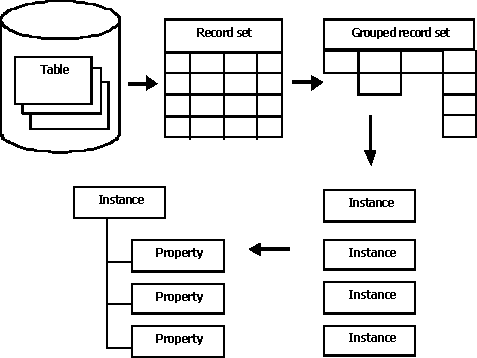
\includegraphics[width=0.75\textwidth]{figures/MappingProcess.pdf}
	\end{center}
	\caption{The D2r mapping process; Taken from \cite{D2rMap_aDatabaseToRdfMappingLanguage}}
	\label{D2rMappingProcessFigure}
\end{figure}

After discussing the SQL to RDF mapping, we look at the keyword search, now:
Mainly there are two possibilities, to implement a keyword search functionality:
\begin{itemize}
	\item {Construct a keyword search query in SQL and let the database answer the query.}
	
	\item {Use a keyword search engine that answers the query based on an external index}
\end{itemize}

At first glance, the first option sounds obviously simple, but after implementing it showed several disadvantages: SQL is not designed to provide search functionality based on keywords. SQL uses the \textbf{\emph{LIKE}} operator for pattern matching. But in order to do a Full-text search, the SQL Query executor cannot use any index resulting in poor query answer performance. Another problem of \emph{LIKE} is, that there is no way to define, that only whole words should be searched and not just sub word matching. Whole word matching is very important, as e.g. a user searching for data about male patients should not also get data about female patients.
As a result, the \emph{LIKE} operator is not suitable for a proper keyword search service as expected to be provided by a dataspace wrapper. Several SQL database vendors provide often own solutions for Full-Text search queries. But these solutions have often other restrictions as e.g. only column fields having the datatype \emph{TEXT} (on MySQL) and the fields have to specified to be fulltext fields, so that the SQL engine is able to create an index for it (at MySQL databases at least).
A Wrapper could use vendor specific services but that would exclude other SQL database vendors, obviously. 

The second option doesn't rise the aforementioned issues of option one. For the Wrapper a keyword searcher was implemented using the fulltext search engine Apache Lucene Core \footnote{\url{https://lucene.apache.org/core/}}. The advantage of using Lucene is it's high-performance and scaling of keyword searches over large data sets. Additionally it allows a fine granular configuration about the query construction and sorts automatically the query result by relevance (so called query result ranking). \\
The major disadvantage of using lucene is that the SQL data have to be extracted and indexed outside the database. If the data changes or rows are added resp. deleted, the index has to be updated accordingly. The update process can be very complex, as not only new data has to be indexed resp. existing data has to be removed, but also data that references the deleted or new data that depends on it.\\
A simpler but obviously slower solution is to reindex the whole data set. Reindexing the whole data set is only advised if updates occur not that often or if it is acceptable if the wrapper updates the index not instantly and thus provides potentially outdated data.

The decision which method is more suitable depends primarily on the use case and the domain. As the project is designed to be used as a test suite for medical datasources and medical science, it is acceptable if the data is outdated to some degree and will be updated not frequently. Changes on the datasource haven't to be updated in near-realtime. Having this in mind, the preferred method for the keyword search functionality clearly is using Apache Lucene Core, as the  advantages clearly outweigh its disadvantages. Thus, a full functional keyword searcher was implemented powered by Lucene.

\subsection{Image Wrapper}
fgfg
\subsection{PDF Wrapper}

\section{Register}

\section{Basic dataspace querying}
\section{Advanced query techniques/features}
\section{GUI}
\section{Validation}

%\include{summaries/summaries}

\chapter{Glossary}

\textbf{Data model} In data modeling theory, a data model is an abstract model that describes how data is represented and used. It consists of a set of data structures and conceptual tools that is used to describe the structure of a database and operations that can be performed on the data. A data model consists of a data model theory, a formal description of the data model, and a data model instance, which is a practical data model designed for a particular application. There exist three types of data models \cite[p.10-14]{IntroductionToDatabaseSystems2010}:
\begin{itemize}
	\item \textbf{Conceptual data model}: Describes data independent from any implementation details. It is used to describe the semantic of a domain. Examples for conceptual data models are the entity-relationship (E-R) model and ontologies. 
	\item \textbf{Logical data model}: Also called representational or implementation data model. Describes data in terms of data structures like relational tables and columns or XML tags. Examples of logical data models are the relational data model, the object-based data model, semi-structured data models like XML or a graph-based data model like RDF. 
	\item \textbf{Physical data model}: Describes data in terms of collection of files, indices and other physical storage structures. It defines how the data is stored on disk and what access methods are available to it. 
\end{itemize}

\textbf{Data source} A data source addresses an arbitrary data storage, whose data should be integrated in an information system. (\cite[p. 7]{DBLP:books/dp/LeserN2006}, own translation)

\textbf{Integrated or integrating information system} An integrated information system is an application, which facilitates the access to different data sources (\cite[p. 7]{DBLP:books/dp/LeserN2006}, own translation)

\textbf{Meta data} Data that describes other data. The distinction between data and meta data in a system, is dependent on the particular application. Meta data has to be stored, browsed and integrated as well as 'normal' data. (\cite[p. 8]{DBLP:books/dp/LeserN2006}, own translation)

\textbf{Schema} The word comes from greek \foreignlanguage{greek}{\emph{σχήμα}}(skhēma) meaning \emph{shape} or \emph{plan}. In computer science the word has different meanings. 
In the context of database theory the word is used for a representation of the structure (syntax), semantics, and constraints on the use of a database (or its portion) in a particular data model. \cite[p. 235]{Sheth:1990:FDS:96602.96604}. Analogous, an XML schema defines the structure, content and semantics of XML documents\cite{w3XMLSchema}. To generalize it, a schema in the context of data integration is the definition of the structure, content and semantics of a data source.




%%%%%%%%%%%%%%%%%%%%%%%%%%%%%%%%%%%%%%
%%% Bibtex-Tool: http://jabref.sourceforge.net/
%%%%%%%%%%%%%%%%%%%%%%%%%%%%%%%%%%%%%%
\bibliographystyle{ieeetr}
\bibliography{bib.bib}
\addcontentsline{toc}{chapter}{\bibname}


\selectlanguage{ngerman}
\begin{center}

\begin{minipage}{.8\textwidth}

\chapter*{Eidesstattliche Erkl"arung}

Ich erkl"are hiermit, dass ich die vorliegende Arbeit selbst"andig verfasst und
keine anderen als die angegebenen Quellen und Hilfsmittel verwendet habe.\\

Die Arbeit wurde bisher keiner anderen Pr"ufungsbeh"orde vorgelegt und auch noch nicht ver"offentlicht.\\

Passau, den 29.03.2018

\vspace{1cm}

David Goeth

\end{minipage}

\end{center}

\clearpage

\end{document}